\section{$^{162}$Dy Results}

$^{162}$Dy, one of the most studied nuclei on the chart of nuclides, with over 24 different reactions and probes (from electron capture, stripping/pickup (t,p)/(p,t) reactions, neutron capture, ($\alpha$,2n) reactions, and ($^3$He,$\alpha$) reactions, to name a few) which have been implemented to extract information on the structure of $^{162}$Dy \cite{Aprahamian200642}. Several previous (n,n$^\prime\gamma$) campaigns were carried out to measure level lifetimes of the isovector M1 scissors mode in $^{162}$Dy (\cite{Yates_162nnp1995}), as well as a series of precision angular distribution measurements by Govor \textit{et.~al} (\cite{Govor_162Dy2002}) to extract multipole mixing fractions and $\gamma$-ray intensities. Analogous to the $^{160}$Gd case study, the angular distributions carried out by Govor act as a complimentary guide and benchmark for our measurements. While the initial and chief goal is to measure the lifetimes of 0$^+$ excitations and low-lying negative parity states, we are also able to populate and measure the lifetimes of the vast majority of low spin (J$<$5) states under the bombarding neutron energy threshold. The full result of all measured lifetimes in the $^{162}$Dy experimental campaign (\S \ref{sec:Dy_exp}) is displayed in the level scheme in Figure \ref{fig:162Dy_All}.

% \begin{center}
% \begin{figure}[h!]
% 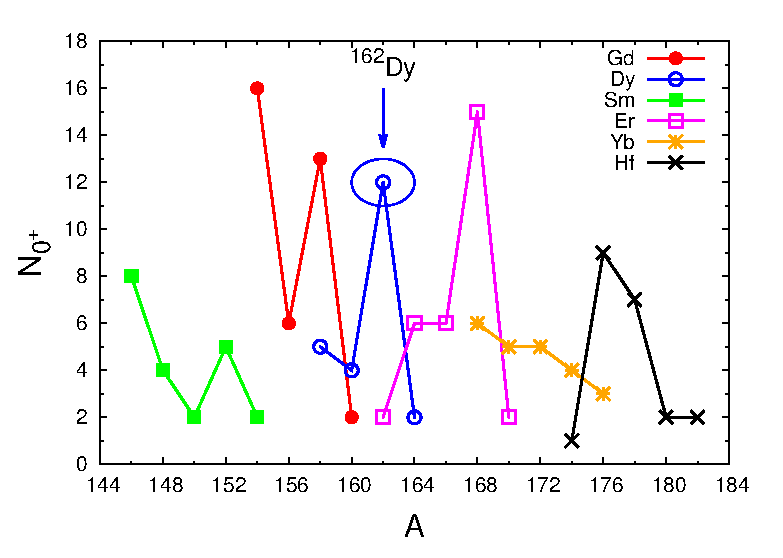
\includegraphics[width=0.90\textwidth]{Gd_Dy_0s_Number.eps}
% \caption{Schematic of the total number of 0$^+$ excitations among several deformed rare-earth nuclei (Sm, Gd, Dy, Er, Yb, and Hf), with emphasis drawn to $^{162}$Dy in a blue circle. \label{fig:RE_0s}}
% \end{figure}
% \end{center}
\begin{landscape}
\begin{figure}[h!]
\begin{center}
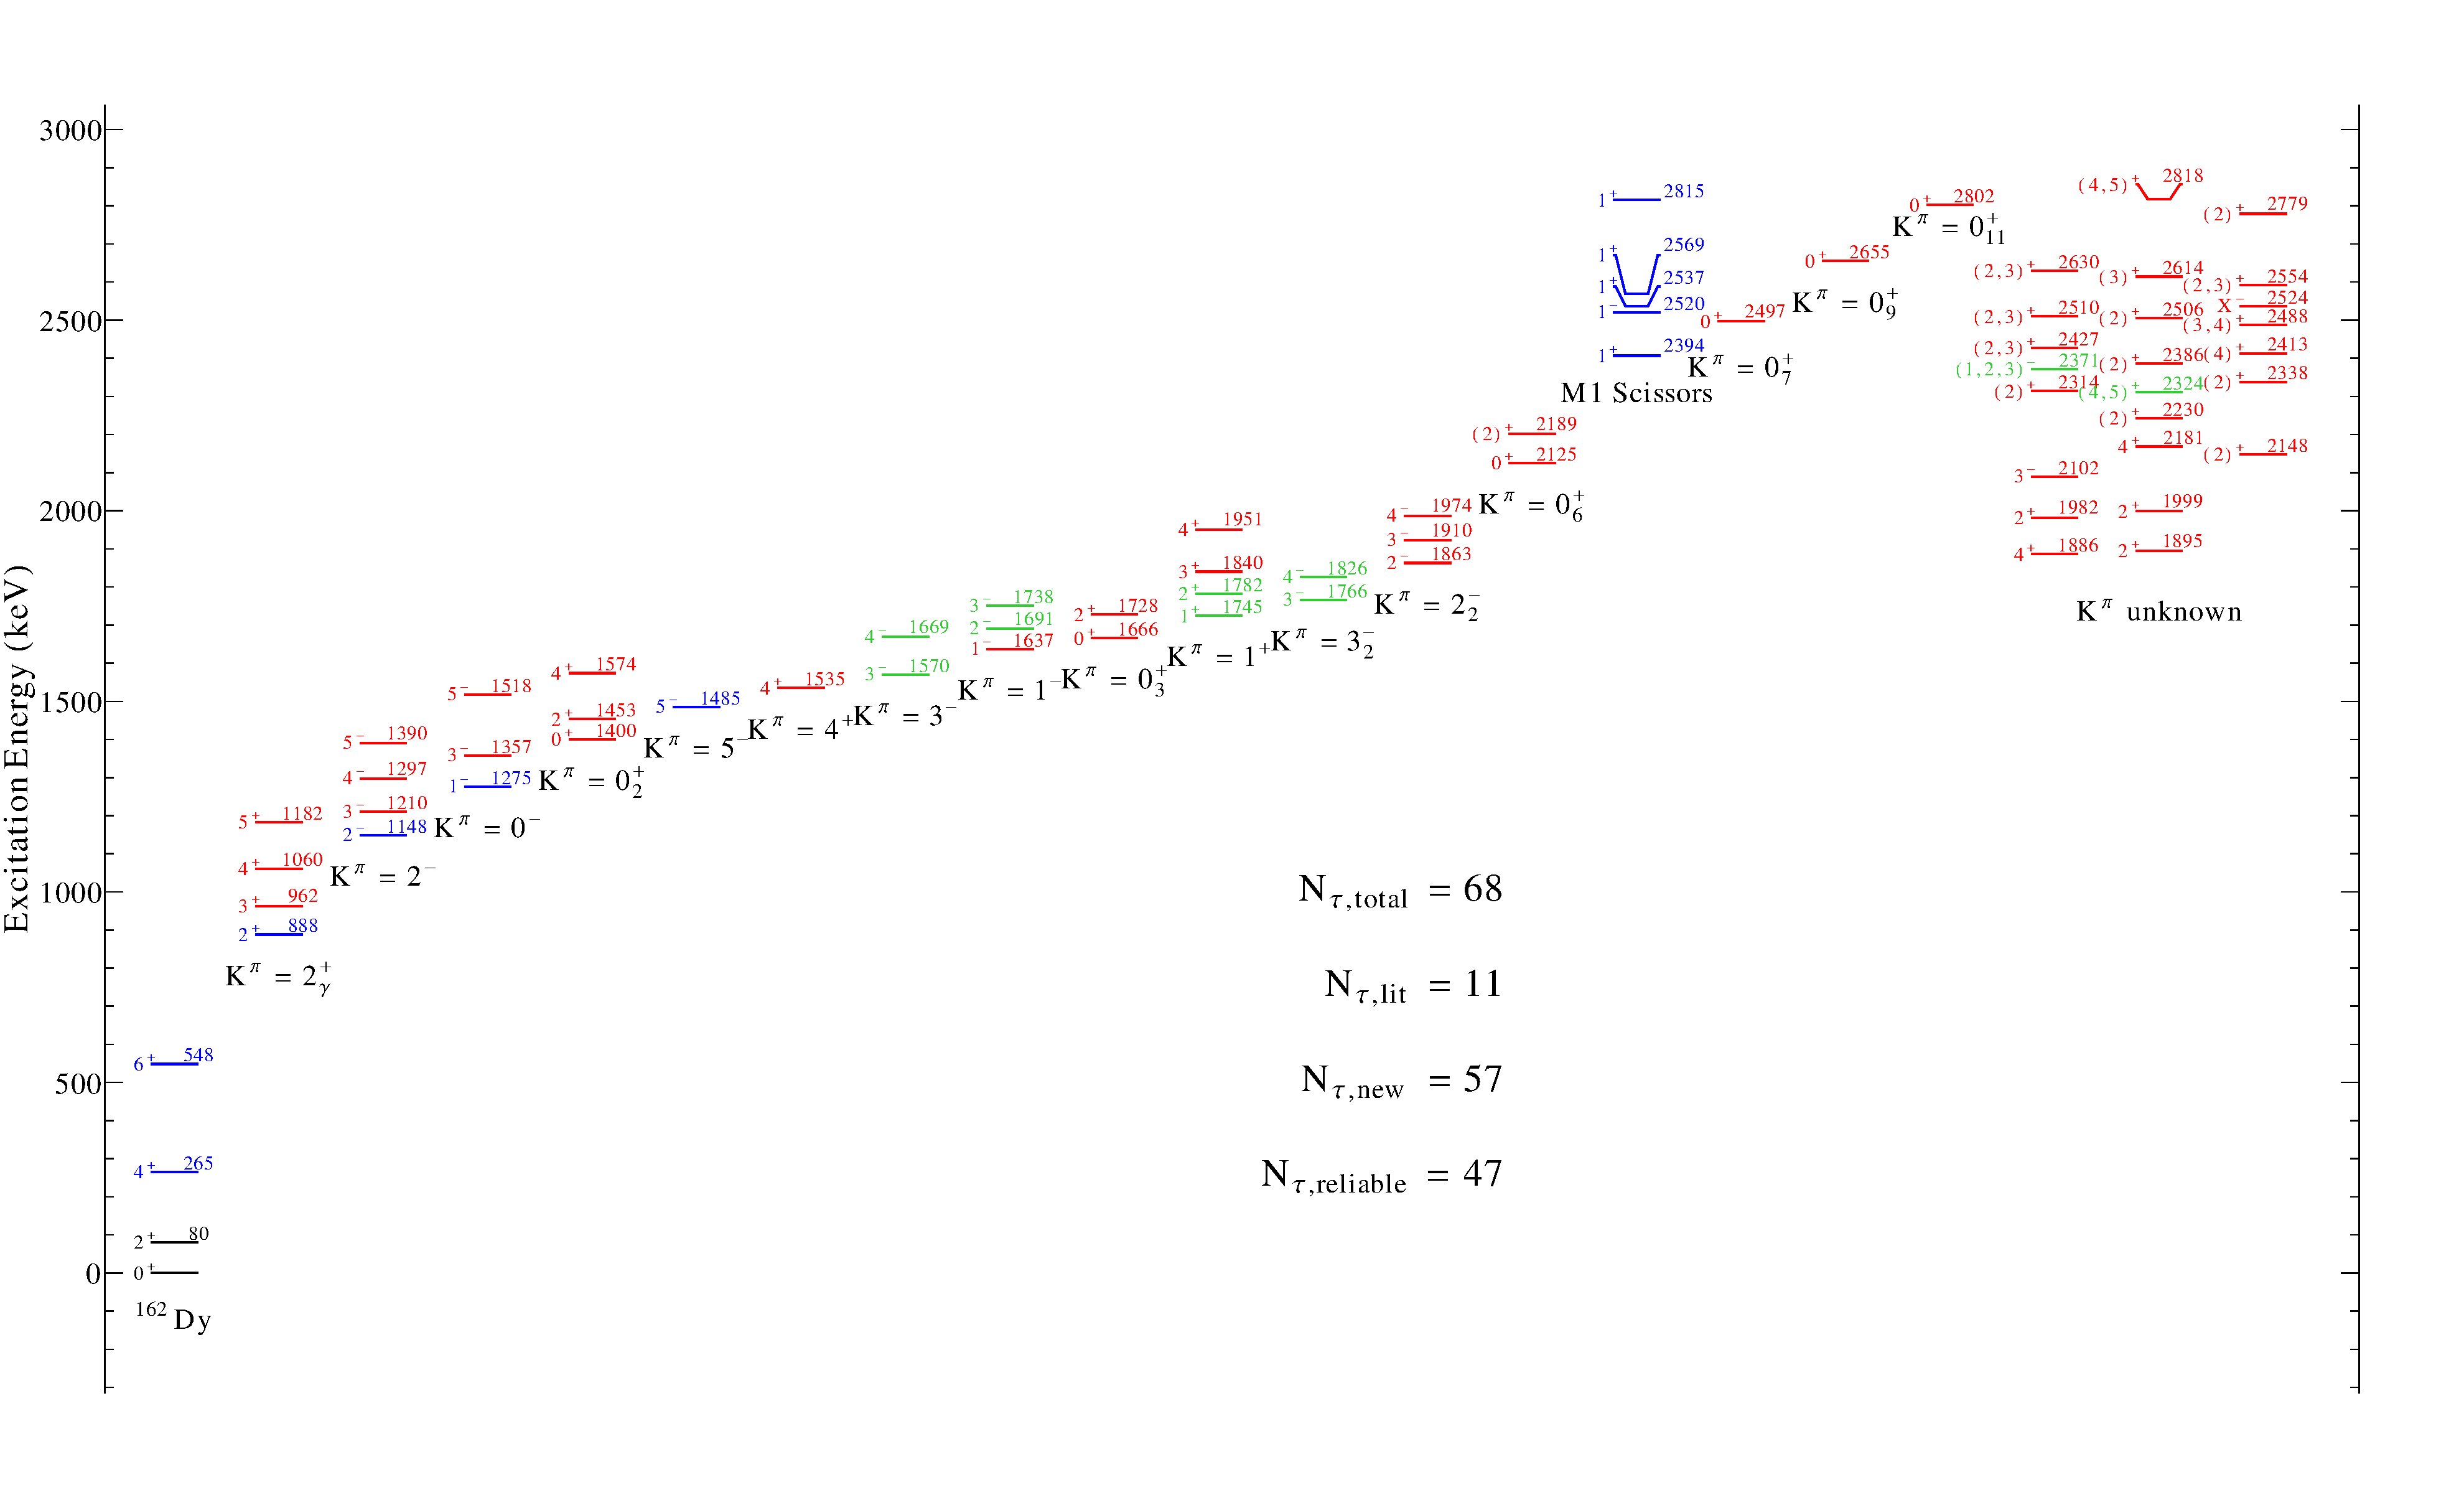
\includegraphics[height=0.8\textheight]{figures/162Dy_All.pdf}
\caption{Level scheme for all level lifetimes measured in the $^{162}$Dy experiments, with confirmed band and spin assignments shown. Previously measured lifetimes are in blue, with newly presented lifetimes in red, levels in green constitute an unreliable lifetime measurement from our data, where F($\tau$)$<$0 or is consistent with zero. 
\label{fig:162Dy_All}}
\end{center}
\end{figure}

\end{landscape}

In Figure \ref{fig:162Dy_All}, levels colored blue are pre-existing lifetimes in literature, where the levels in red are newly presented lifetime measurements in this work. Due to the limitations of DSAM outlined in \S \ref{sec:AD_Ft}, cases where F($\tau$) is strictly less than zero or consistent with 0 within 1$\sigma$, unreliable lifetimes are colored green. Again, it must be reiterated that while these lifetimes do not have previously measured literature values, our (n,n$^\prime\gamma$) lifetimes should not be trusted as a good measurement. Other techniques must be implemented to fully measure the lifetime of these states (Coulomb Excitation, RDDM plunger method, etc). Excitations are placed into bands where available, along with the well-measured and studied isovector M1 scissors mode lifetimes at $\sim$2.4~MeV that results in J$^\pi$=1$^{\pm}$ excitations \cite{Margraf_gg'NRF_1995, WESSELBORG198822,Yates_162nnp1995}. In total, we observed 108 discrete $\gamma$-rays to measure sixty eight (68) lifetimes, fifty seven (57) of which were measured for the first time. Of the newly measured lifetimes, however, only forty seven (47) are considered reliable from our measurement of Doppler energy shifted $\gamma$ rays. These measured lifetimes were extracted from the three angular distribution measurements (E$_n$=1.6, 2.2, \& 3.1~MeV), with three effective ranges of lifetime sensitivity, in the hopes of limiting any lifetime feeding from higher levels and bombarding neutron energy. Visually, the ranges of lifetimes reported can be seen in Figure \ref{fig:162Dy_viz_lifetimes}, where we have a comparison of the presented lifetimes (and corresponding errors) in to literature lifetimes in the three separate ranges of lifetime sensitivity (excitation energies of $<$1.6~MeV in red, 1.6~-~2.2~MeV in green, and 2.2~MeV~-~3.1~MeV in blue). 


\begin{table}[h!]
\begin{center}
\caption{LITERATURE LIFETIME COMPARISON: $^{162}$DY \label{tab:lifetimes_comparison}}
% \makebox[\textwidth]{
\begin{tabular}{c|c|c}
E$_{lev}$ (keV) & $\tau_{(n,n^\prime\gamma)}$ (fs) & $\tau_{lit}$ (fs) \\
\hline
\hline
265  & $>$1500[$\dagger$]      & 0.190E6 (7) [$\oplus$] \\
548  & $>$960[$\dagger$]       & 26.5E3 (14) [$\oplus$] \\
888  & $>$3700                 & 2840 (3) [$\oplus$] \\
1148 & 2100$^{+7200}_{-1200}$  & 0.30E6 (6) [$\ominus$]\\
1275 & 120$^{+10}_{-10}$   & 28.8 (6) [$\ddagger$][$\oplus$]\\
1485 & 400$^{+210}_{-140}$ & 2.76E6 (16) [$\ddagger$][$\otimes$]\\
2394 & 14$^{+13}_{-11}$    & 16$^{+10}_{-10}$ [$\Omega$]\\
2520 & 110$^{+30}_{-20}$   & 11$^{+9}_{-9}$ [$\Omega$]\\
2537 & 460$^{+160}_{-120}$ & 141$^{+30}_{-30}$ [$\Omega$]\\
2569 & 90$^{+30}_{-20}$    & 56$^{+6}_{-6}$ [$\Omega$]\\
2815 & 200$^{+130}_{-60}$  & 56$^{+19}_{-19}$ [$\Omega$] \\
\end{tabular}\\ \vspace{10pt}
\end{center}
Comparison of lifetimes measured in the campaign of $^{162}$Dy(n,n$^\prime\gamma$) experiments with literature lifetimes.
[$\dagger$]: Measured lifetime not reliable (F($\tau$) within 1$\sigma$ of 0) - resulting lifetimes fall well outside the range of DSAM.
[$\ddagger$]: Lifetime called into question in this work. 
[$\ominus$]: from $^{162}$Tb $\beta^-$ decay \cite{PhysRev.166.1227}.
[$\otimes$]: from $^{162}$Ho $\varepsilon$-decay \cite{Honig_5minus1969}. 
[$\oplus$]: from B(E2)$\uparrow$ via Coul. Ex \cite{GROTDAL1968385}. 
[$\Omega$]: from ($\gamma$,$\gamma^\prime$) \cite{Margraf_gg'NRF_1995} and (n,n$^\prime\gamma$) \cite{Yates_162nnp1995}
% \end{center}
\end{table}

% \begin{figure}[h!]
% \begin{center}
% \includegraphics[width=0.95\textwidth]{162Dy_viz_lifetimes.eps}
% \caption{Visual representation of all measured lifetimes with respect to literature values (in black). Each separate color outlines the specific regimes ($<$1.6~MeV (in red), 1.6~-~2.2~MeV (in green), and 2.2~MeV~-~3.1~MeV (in blue) excitation energy) of energies studied in the $^{162}$Dy angular distributions. \label{fig:162Dy_lifetimes}}
% \end{center}
% \end{figure}

The discrepancies from the literature lifetimes are clearly visible in Figure \ref{fig:162Dy_viz_lifetimes}, where we can attribute slight inflation of the lifetimes as a result of either feeding from higher-lying states, or from the bombarding neutron energy effects mentioned at the beginning of \S \ref{sec:lifetime_inflation}. We can make the justification that our lifetimes agree reasonably with literature because the accuracy of measurement is roughly on the same order of magnitude for every sensitive range of lifetimes measured, with scattered cases of good agreement. In other words, the lifetimes measured at intermediate energies ($\sim$900~keV, $\sim$1850~keV, and $\sim$2400~keV) are inflated by the same proportional amount for each bombarding neutron energy. Further discrepancies in our measured lifetimes to those in literature stem from the differences in measurement techniques (DSAM-INS versus deduction of lifetimes via direct B(E1/M1)$\uparrow$). For example, the weighted average of the F($\tau$) values for multi-channel decays out of a state can result in a lower average F($\tau$) if only one $\gamma$-ray decay is used in the determination of the lifetime, resulting in a longer lifetime. 

\begin{figure}[h!]
\begin{center}
\includegraphics[width=0.999\textwidth]{figures/162Dy_viz_lifetimes.eps}
\caption{All measured lifetimes in $^{162}$Dy (in femtoseconds) plotted as a function of excitation energy in keV. Data points in red are extracted from the E$_n$=1.6~MeV angular distributions, points in green correspond to lifetimes extracted from the 2.2~MeV angular distributions, and blue points are lifetimes from the 3.1~MeV dataset. (color online) \label{fig:162Dy_viz_lifetimes}}
\end{center}
\end{figure}

An example of the E$_n$=2.2~MeV angular distribution singles-spectrum for $^{162}$Dy(n,n$^\prime\gamma$) can be seen in Figure \ref{fig:162Dy_220_spectrum} with select peaks labeled for reference.

\begin{figure}[h!]
\begin{center}

\includegraphics[width=0.95\textwidth]{figures/sample_spec_stacked_220.eps}
\caption{Singles spectra from the $\theta_{lab}$=90$^\circ$ and E$_n$=2.2~MeV angular distributions of $^{162}$Dy. \label{fig:162Dy_220_spectrum}}
\end{center}
\end{figure}

%visualization and preface to results (overview)
\subsection{Lifetimes of 0$^+$ States}
In stark contrast to the results of the $^{160}$Gd experiments (namely the lower limit lifetimes and existence of anisotropies in angular distributions), we are able to determine definite level lifetimes for the majority of 0$^+$ bands and confirm isotropic angular distributions from the $^{162}$Dy data. DSAM plots and angular distributions for the full 0$^+_i\rightarrow$2$^+_{g.s.}$ de-excitations are seen in Figures \ref{fig:162Dy_0s_FT} and \ref{fig:162Dy_0s_AD}, respectively. We also do not exclude any of the proposed 0$^+$ states from our observation of isotropic or anisotropies in the angular distributions similar to our $^{160}$Gd results.

\begin{figure}[h!]
\begin{center}
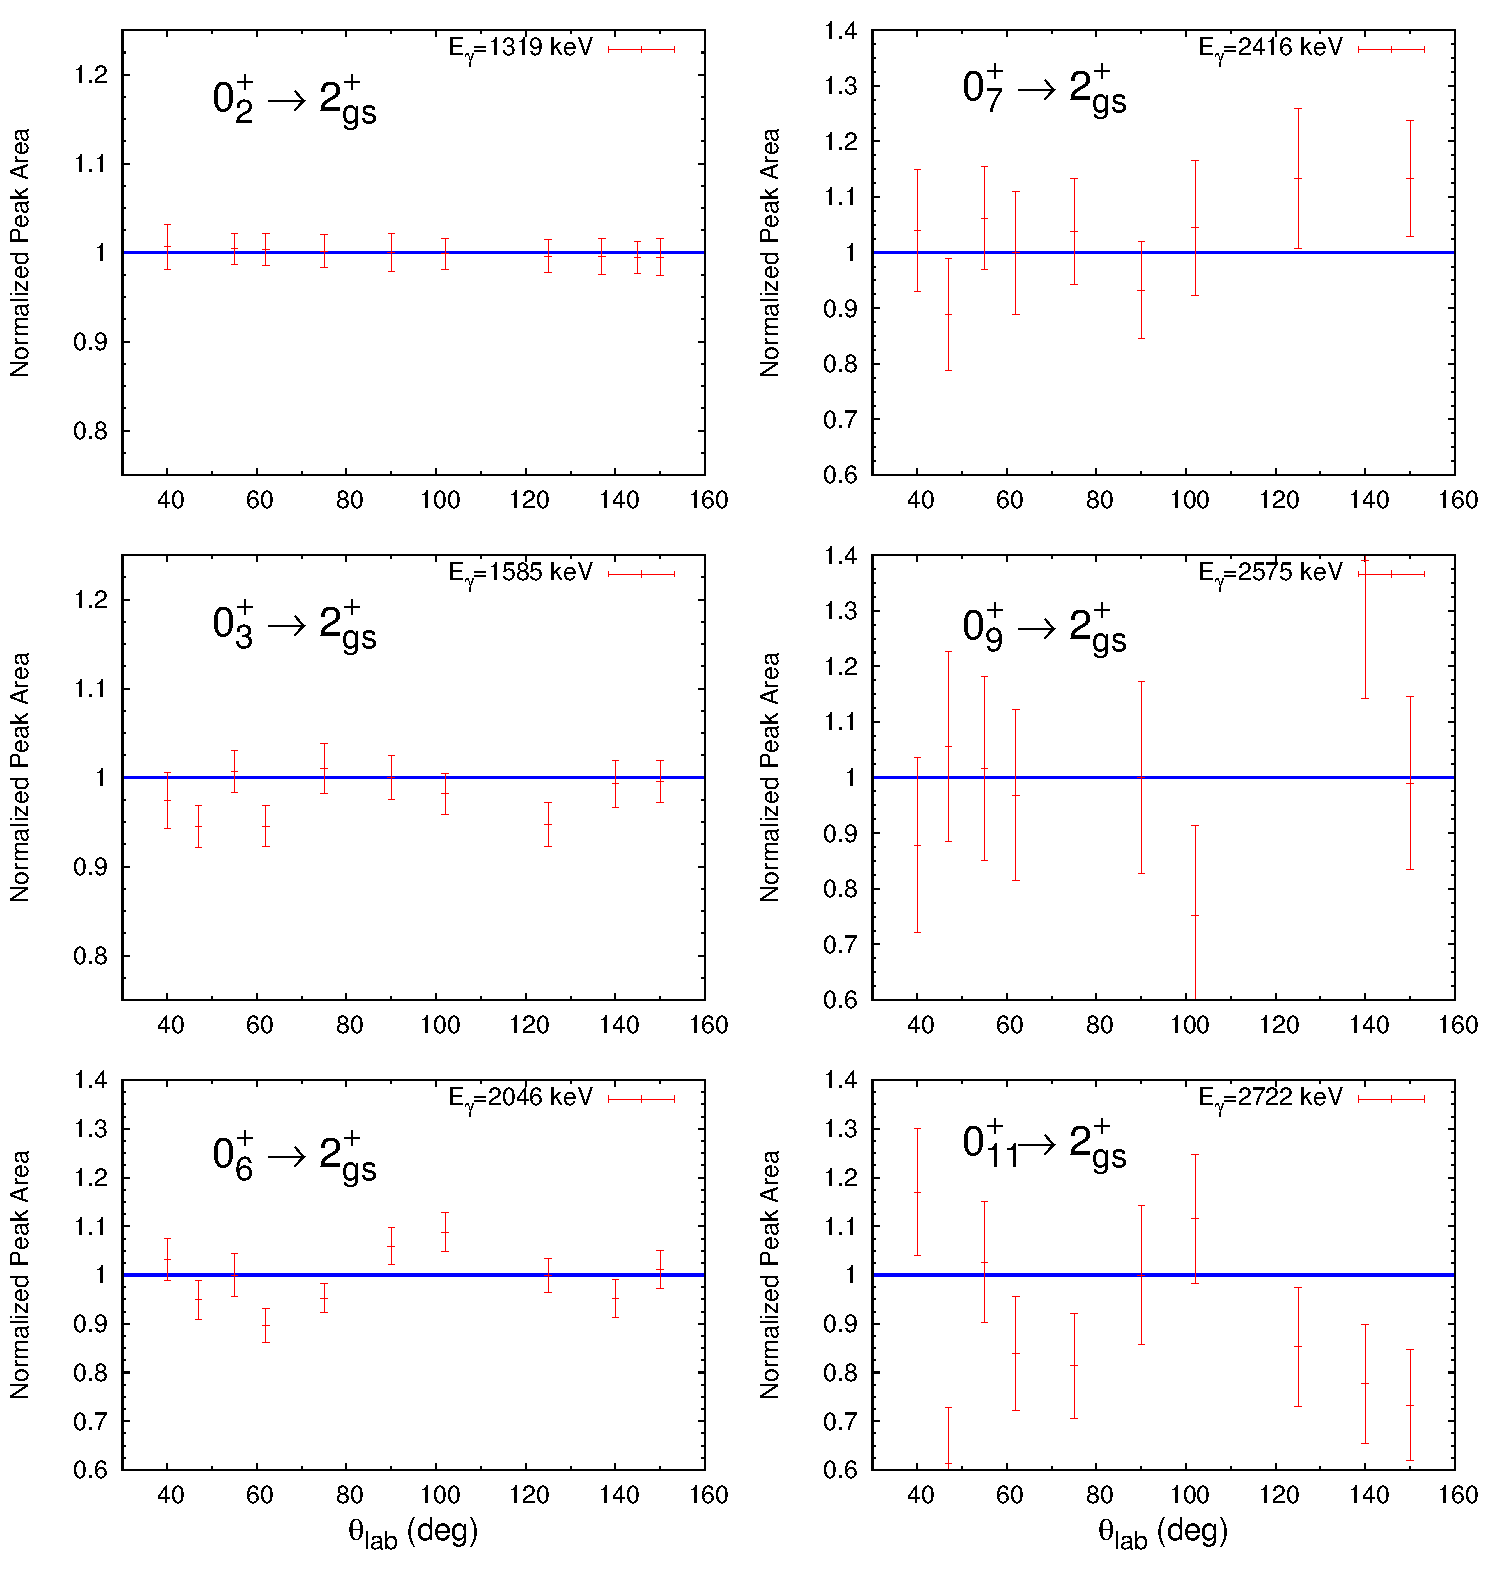
\includegraphics[width=0.95\textwidth]{figures/162Dy_0s_AD.pdf}
\caption{Angular distributions of 0$^+_i\rightarrow$2$^+_{g.s.}$ $\gamma$-rays observed in $^{162}$Dy, highlighting their isotropic nature (color online). \label{fig:162Dy_0s_AD}}
\end{center}
\end{figure}

\begin{figure}[h!]
\begin{center}
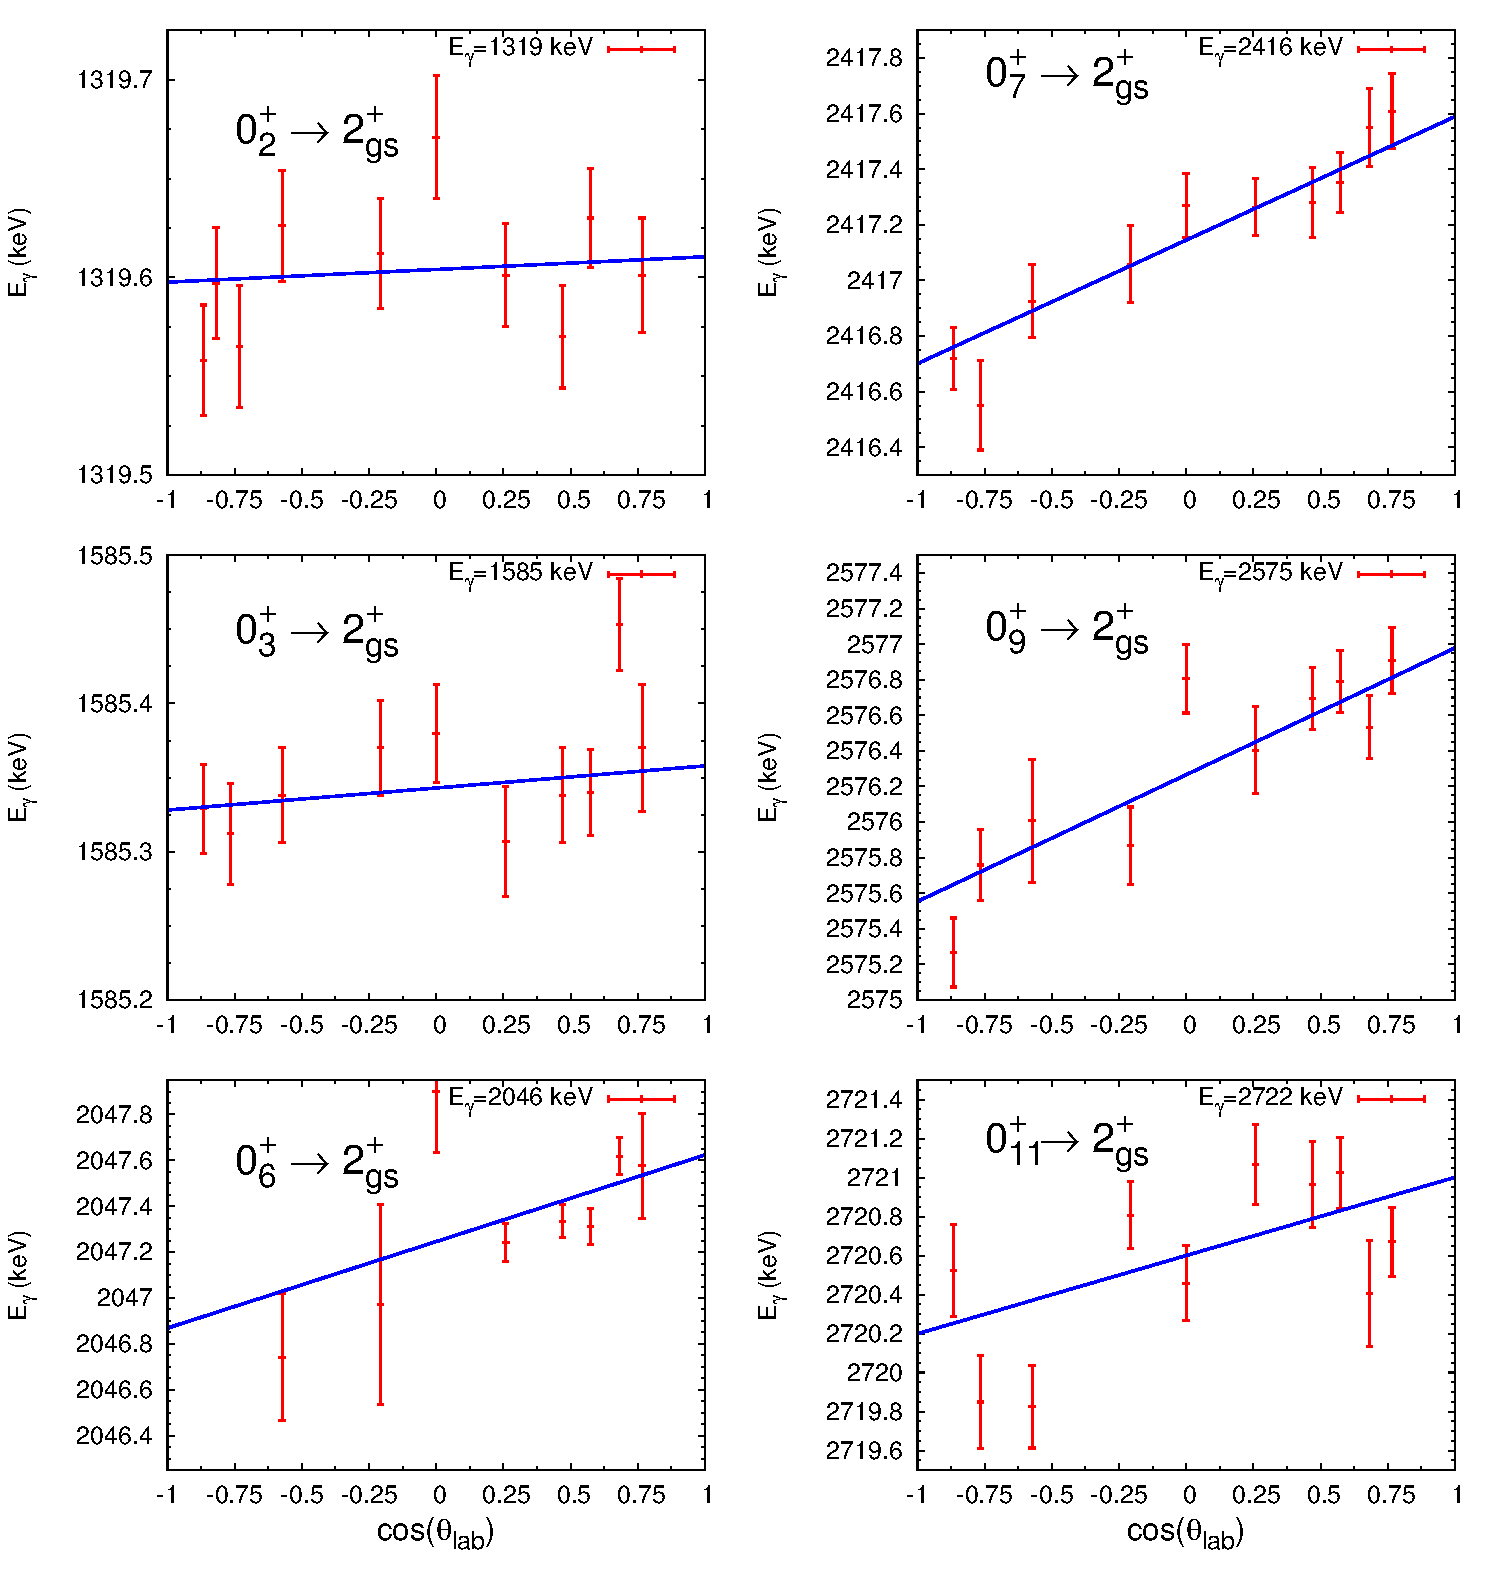
\includegraphics[width=0.95\textwidth]{figures/162Dy_0s_FT.pdf}
\caption{Doppler energy shifts of 0$^+_i\rightarrow$2$^+_{g.s.}$ $\gamma$-rays observed in $^{162}$Dy (color online). \label{fig:162Dy_0s_FT}}
\end{center}
\end{figure}

Lifetimes for six (6) of the eleven (11) confirmed and tentative excited 0$^+$ states \cite{Meyer_pt0_2006} were measured in the campaign of experiments (shown in Table \ref{tab:0s_comparison}). We have also measured lifetimes (including a few lower limits) of the five lowest-lying rotational members of the K$^\pi$=2$^+$ band, the bandheads of both K$^\pi$=4$^+$ bands, and a total of 52 other states in $^{162}$Dy. The absolute intensities of decays discussed in this work were extracted from the angular distributions and are shown in Table \ref{tab:162Dy_multiphonon_intensities}, with unobserved transition intensities taken from literature \cite{Aprahamian200642,Zamfir_162Dy0_1999,Wu_2minus_2001} to provide pertinent discussion later in this manuscript.


The full tabulation of $\gamma$ decays observed for the de-excitation of K$^\pi$=0$^+$ bands is shown in Table \ref{tab:162Dy_0s_all}, which includes experimentally measured lifetimes in femtoseconds, branching ratios, and $\gamma$-ray energies in keV. Mixed multipolarity de-excitations are assigned a multipole mixing fraction ($\delta_{mixing}$) from comparison of our gathered angular distributions to a statistical model calculation, performed with {\tt CINDY} \cite{SHELDON197399}. A level scheme outlining all observed decays from 0$^+$ bands to the ground state band is also shown in Figure \ref{fig:162Dy_0s_all}.

Lifetimes for the three lowest-lying rotational members of the 0$^+_2$ band were measured; the single, most intense $\gamma$ ray at 1319~keV was used to measure (a shallow) F($\tau$) to extract the lifetime from the E$_n$=1.6~MeV dataset. The weighted average of F($\tau$) from both the 1187 \& 1372~keV $\gamma$ ray is used to measure the lifetime of the 2$^+$ state. Only the 1308~keV de-excitation contributes to the lifetime of the 4$^+$ state at E$_{\rm x}$=1574~keV, as the 1025~keV transition exhibits a negative F($\tau$) value.

We have measured the lifetime of the bandhead and 2$^+$ member of the 0$^+_3$ band at E$_{\rm x}$=1666~keV, with good lifetime resolution extracted from the E$_n$=2.2~MeV dataset. The single 1585~keV transition from the bandhead to the ground state yields a 3000$^{+4800}_{-1300}$~fs lifetime, while only the 1647 and 1728~keV $\gamma$ rays offer contributions to the 2$^+$ lifetime of 1800$^{+880}_{-430}$~fs, as the decay at 1462~keV is coincident with a background line, making that particular F($\tau$) unreliable. Large uncertainties exist for the bandhead of this 0$^+$ band due to the natural limits of lifetimes measurable with DSAM; this large error stems from the uncertainties on the measured F($\tau$) value.

We adopt the placement \cite{BERZINS1995413} of the (2$^+$) state at 2189~keV as the 2$^+$ rotational band member of the 0$^+_6$ band at E$_{\rm x}$=2128~keV, and have measured lifetimes for these two states from the single-channel decays of 2109 \& 2047~keV, respectively. The lifetime of the bandhead was found to be 2300$^{+1500}_{-860}$~fs, and 530$^{+220}_{-160}$~fs for the 2$^+$ member.

The seventh and ninth 0$^+$ states decay via full energy de-excitations to the ground state at E$_\gamma$=2417 \& 2575~keV, respectively. These corresponding lifetimes extracted from the E$_n$=3.1~MeV dataset are 270$^{+110}_{-60}$~fs for the 0$^+$ state at 2497~keV, and 210$^{+300}_{-100}$~fs at 2655~keV. 

Due to the isotropic radiation observed for the 2721~keV $\gamma$-ray that depopulates the (0$^+_{11}$) state at 2802~keV, we support the assignment of this state as a 0$^+$ excitation, where further mentions of this state are considered as a confirmed 0$^+$ state. The Doppler shift from this 2721~keV decay gives us our shortest 0$^+$ lifetime of 90$^{+110}_{-60}$~fs.

\begin{landscape}
\begin{center}
% \begin{table}[h!]
\begin{longtable}{cllcccllll}
% \begin{center}
\caption{K$^\pi$=0$^+$ BANDS: $^{162}$DY \label{tab:162Dy_0s_all}}\\

% \resizebox{1.15\textwidth}{!}{
% \begin{tabular}{cllcccllll}
K$^\pi$                         & E$_{level}$ (keV) & E$_\gamma$ (keV) & J$^\pi_{K^\pi_i}$ & J$^\pi_{K^\pi_f}$ & F($\tau$)$_{av}$ & $\tau$ (fs)                       & BR             & $\pi\ell$         & B($\pi\ell$) (W.u.) \\ \hline \hline \endfirsthead
\caption[]{K$^\pi$=0$^+$ BANDS: $^{162}$DY}{Continued}\\
K$^\pi$                         & E$_{level}$ (keV) & E$_\gamma$ (keV) & J$^\pi_{K^\pi_i}$ & J$^\pi_{K^\pi_f}$ & F($\tau$)$_{av}$ & $\tau$ (fs)                       & BR             & $\pi\ell$         & B($\pi\ell$) (W.u.) \\ \hline \hline \endhead
\underline{K$^\pi$=0$^+_2$:}    & 1400.29(36)  & 512.0(2)                   & 0$^+_{0^+_2}$    & 2$^+_{2^+_1}$ &0.031$\pm$0.038& $>$2100$^{[\vartheta]}$                 & $^{[\dagger]}$ & E2                & ($<$16) \\
                                &              & 1319.60(51)                & 0$^+_{0^+_2}$    & 2$^+_{0^+_1}$ &&                                                     & 1.000          & E2                & $<$1.9   \\
                                & 1453.50(30)  & 395.49 (10)                & 2$^+_{0^+_2}$    & 4$^+_{2^+_1}$ &0.042$\pm$0.026& 3400$^{+5600}_{-1300}$ $^{[\vartheta]}$ & $^{[\dagger]}$ & E2                & (2.7$^{+1.7}_{-1.7}$) \\
                                &              & 565.32 (12)                & 2$^+_{0^+_2}$    & 2$^+_{2^+_1}$ &&                                                     & $^{[\dagger]}$ & E2$^{[\ddagger]}$ & (0.9$^{+0.6}_{-0.6}$) \\
                                &              & 1187.81(51)                & 2$^+_{0^+_2}$    & 4$^+_{0^+_1}$ &&                                                     & 0.425(4)       & E2                & 0.8$^{+0.5}_{-0.5}$                         \\
                                &              & 1372.80(51)                & 2$^+_{0^+_2}$    & 2$^+_{0^+_1}$ &&                                                     & 0.575(4)       & E2/M1$^{[a\varsigma]}$& 0.3$^{+0.2}_{-0.2}$ \\  
                                & 1574.34(29)  & 513.31 (2)                 & 4$^+_{0^+_2}$    & 4$^+_{2^+_1}$ &0.043$\pm$0.031& $>$2000$^{[\varsigma]}$                  & $^{[\dagger]}$ & E2$^{[\ddagger]}$ & ($<$3.7) \\
                                &              & 611.23 (5)                 & 4$^+_{0^+_2}$    & 3$^+_{2^+_1}$ &&                                                     & $^{[\dagger]}$ & E2$^{[\ddagger]}$ & ($<$0.4) \\
                                &              & 686.15 (6)                 & 4$^+_{0^+_2}$    & 2$^+_{2^+_1}$ &&                                                     & $^{[\dagger]}$ & E2                & ($<$0.5) \\
                                &              & 1025.84(58)$^{[\oslash]}$  & 4$^+_{0^+_2}$    & 6$^+_{0^+_1}$ &&                                                     & 0.157(5)       & E2                & $<$1.1   \\
                                &              & 1308.65(51)                & 4$^+_{0^+_2}$    & 4$^+_{0^+_1}$ &&                                                     & 0.843(5)       & E2/M1$^{[b,\varsigma]}$& $<$0.8   \\          \hline
\underline{K$^\pi$=0$^+_3$:}    & 1666.01(33)  & 1585.35(51)                & 0$^+_{0^+_3}$    & 2$^+_{0^+_1}$ &0.051$\pm$0.033 & 3000$^{+4800}_{-1300}$ $^{[\varsigma]}$ & 1.000          & E2                & 0.5$^{+0.4}_{-0.3}$   \\
                                & 1728.31(20)  & 1462.70(51)$^{[\otimes]}$ & 2$^+_{0^+_3}$    & 4$^+_{0^+_1}$ &0.081$\pm$0.023& 1800$^{+880}_{-430}$ $^{[\varsigma]}$    &0.334(5)$^{[\star]}$ & E2           & 0.4$^{+0.1}_{-0.1}$ \\   
                                &              & 1647.64(51)                & 2$^+_{0^+_3}$    & 2$^+_{0^+_1}$ &&                                                     &0.407(5)        & E2/M1$^{[c,\varsigma]}$& 0.01$^{+0.01}_{-0.01}$ \\   
                                &              & 1728.29(53)                & 2$^+_{0^+_3}$    & 0$^+_{0^+_1}$ &&                                                     &0.259(4)        & E2                & 0.2$^{+0.1}_{-0.1}$  \\ \hline   
\underline{K$^\pi$=0$^+_6$:}    & 2128.02(33)  & 2047.34(61)                & 0$^+_{0^+_6}$    & 2$^+_{0^+_1}$ &0.071$\pm$0.031& 2300$^{+1500}_{-860}$ $^{[\varpi]}$ &1.000           & E2                & 0.2$^{+0.1}_{-0.1}$       \\  
                                & 2189.65(52)  & 2109.10(50)                & (2)$^+_{0^+_{6}}$& 2$^+_{0^+_1}$ &0.267$\pm$0.058& 530$^{+220}_{-160}$ $^{[\varpi]}$   &1.000           &(E2/M1)$^{[d,\varpi]}$    & 0.7$^{+0.3}_{-0.2}$   \\  \hline
\underline{K$^\pi$=0$^+_7$:}    & 2497.77(52)  & 2417.22(50)                & 0$^+_{0^+_7}$    & 2$^+_{0^+_1}$ &0.376$\pm$0.055& 270$^{+110}_{-60}$ $^{[\varpi]}$    &1.000           & E2                & 0.7$^{+0.2}_{-0.2}$     \\ \hline
\underline{K$^\pi$=0$^+_9$:}    & 2655.83(33)  & 2575.28(53)                & 0$^+_{0^+_9}$    & 2$^+_{0^+_1}$ &0.436$\pm$0.164& 210$^{+300}_{-100}$ $^{[\varpi]}$   &1.000           & E2                & 0.7$^{+0.6}_{-0.4}$       \\ \hline
\underline{K$^\pi$=0$^+_{11}$:} & 2802.04(61)  & 2721.48(55)                & 0$^+_{0^+_{11}}$ & 2$^+_{0^+_1}$ &0.653$\pm$0.200& 90$^{+110}_{-60}$ $^{[\varpi]}$     &1.000           & E2                & 1.2$^{+2.3}_{-0.6}$      \\ \hline
 
% \end{tabular}

\vspace{10pt}
\end{longtable}
\end{center}
Lifetimes of excited 0$^+$ bands in $^{162}$Dy, with calculated B(E2) in W.u., from our measured multipole mixing fractions, branching ratios, $\gamma$-ray energies, and lifetimes, all extracted from the angular distributions. B(E2) strengths in parentheses are calculated using literature intensities.\\
 $^{[a]}$: $\delta$=1.3$^{+0.2}_{-0.2}$,
 $^{[b]}$: $\delta$=0.93$^{+0.14}_{-0.15}$,
 $^{[c]}$: $\delta$=-0.22$^{+0.08}_{-0.08}$,
 $^{[d]}$: $\delta$=2.7$^{+1.8}_{-0.9}$\\
 $^{[\dagger]}$: Intensity information taken from \cite{Aprahamian200642,Zamfir_162Dy0_1999} ($\gamma$-ray not seen in this work),
 $^{[\ddagger]}$: Mixing information not available, full E2 strength reported,
 $^{[\oslash]}$: $\gamma$ ray not used in F($\tau$) calculation (F($\tau$)$<$0).\\
 $^{[\vartheta]}$: F($\tau$) or $\delta_{mixing}$ extracted from E$_n$=1.6~MeV angular distributions,
 $^{[\varsigma]}$: F($\tau$) or $\delta_{mixing}$ extracted from E$_n$=2.2~MeV angular distributions,
 $^{[\varpi]}$: F($\tau$) or $\delta_{mixing}$ extracted from E$_n$=3.1~MeV angular distributions,
 $^{[\otimes]}$: $\gamma$ ray coincident with background, not used in calculation of lifetime.\\
 1~W.u.=5.25E-7~e$^2$b$^2$
% \end{center}
% \end{table}
% \end{longtable}
% \end{center}
\end{landscape}

\subsection{Lifetimes of K$^\pi$=2$^+_\gamma$ and 4$^+$ Bands}

In the eight decays from the 2$^+$ band, two of the $\gamma$ rays (the 697~keV and 634~keV de-excitations) are not used in the calculation of the level lifetime, as they have Doppler shifts that correspond to an F($\tau$)$<$0. Lower limits for the lifetime are measured in several cases due to the inherent limitations of sensitive lifetimes DSAM can measure (up to a few picoseconds).


% \begin{table}[h!]
\begin{landscape}
\begin{center}
\begin{longtable}{cllcccllll}
\caption{K$^\pi$=2$^+$ AND 4$^+$ BANDS: $^{162}$DY \label{tab:162Dy_gamma_doublegamma}}\\ % \resizebox{1.15\textwidth}{!}{
% \begin{tabular}{cllcccllll}
K$^\pi$                           & E$_{level}$ (keV) & E$_\gamma$ (keV)     & J$^\pi_{K^\pi_i}$  & J$^\pi_{K^\pi_f}$  &F($\tau$)$_{av}$ & $\tau$ (fs)                        & BR        & $\pi\ell$     & B($\pi\ell$) (W.u.) \\ \hline \hline \endfirsthead
\caption[]{K$^\pi$=2$^+$ AND 4$^+$ BANDS: $^{162}$DY}{Continued}\\ % \resizebox{1.15\textwidth}{!}{
% \begin{tabular}{cllcccllll}
K$^\pi$                           & E$_{level}$ (keV) & E$_\gamma$ (keV)     & J$^\pi_{K^\pi_i}$  & J$^\pi_{K^\pi_f}$  &F($\tau$)$_{av}$ & $\tau$ (fs)                        & BR        & $\pi\ell$     & B($\pi\ell$) (W.u.) \\ \hline \hline \endhead
\underline{K$^\pi$=2$^+_\gamma$:} &  888.18(22) &  807.54(50)               & 2$^+_{2^+_\gamma}$ & 2$^+_{0^+_1}$ &0.022$\pm$0.018& $>$3700 $^{[\vartheta]}$                       & 0.524(3)            & E2/M1$^{[a,\vartheta]}$  & $<$1.1 \\
                                  &             &  888.18(50)               & 2$^+_{2^+_\gamma}$ & 0$^+_{0^+_1}$ &&                                                            & 0.476(3)            & E2                    & $<$3.6                            \\ 
                                  &  962.96(27) &  697.30(50)$^{[\oslash]}$ & 3$^+_{2^+_\gamma}$ & 4$^+_{0^+_1}$ &0.021$\pm$0.025& $>$3200 $^{[\vartheta]}$                       & 0.159(3)            & E2/M1$^{[b,\vartheta]}$  & $<$0.2    \\
                                  &             &  882.31(50)               & 3$^+_{2^+_\gamma}$ & 2$^+_{0^+_1}$ &&                                                            & 0.841(3)            & E2/M1$^{[c,\vartheta]}$  & $<$7.6                  \\ 
                                  & 1061.05(29) &  795.35(50)               & 4$^+_{2^+_\gamma}$ & 4$^+_{0^+_1}$ &0.047$\pm$0.030& 3200$^{+4800}_{-1300}$ $^{[\vartheta]}$        & 0.637(3)            & E2/M1$^{[d,\vartheta]}$  & 4.5$^{+2.7}_{-3.1}$ \\
                                  &             &  980.36(51)               & 4$^+_{2^+_\gamma}$ & 2$^+_{0^+_1}$ &&                                                            & 0.363(3)            & E2                    & 2.0$^{+1.3}_{-1.2}$             \\ 
                                  & 1182.88(26) &  634.24(61)               & 5$^+_{2^+_\gamma}$ & 6$^+_{0^+_1}$ &0.034$\pm$0.030& $>$2500 $^{[\varsigma]}$                        &0.239(5)             & E2/M1$^{[e,\vartheta]}$  & $<$14   \\
                                  &             &  917.18(51)               & 5$^+_{2^+_\gamma}$ & 4$^+_{0^+_1}$ &&                                                            &0.761(5)             & E2/M1$^{[f,\vartheta]}$  & $<$7.3   \\ \hline
\underline{K$^\pi$=4$^+_1$:}      & 1535.97(23) &  475.27(54)$^{[\otimes]}$& 4$^+_{4^+_1}$& 4$^+_{2^+_\gamma}$ &0.124$\pm$0.077& 1200$^{+2100}_{-450}$ $^{[\varsigma]}$           &0.186(10)$^{[\star]}$& E2/M1$^{[g,\varsigma]}$    & 44$^{+34}_{-40}$ (23$^{+18}_{-21}$)       \\
                                  &             &  572.96(50)               & 4$^+_{4^+_1}$& 3$^+_{2^+_\gamma}$ &&                                                             &0.317(6)             & E2/M1$^{[h,\varsigma]}$    & 66$^{+42}_{-40}$ (98$^{+63}_{-59}$)       \\
                                  &             &  647.61(50)$^{[\oslash]}$ & 4$^+_{4^+_1}$& 2$^+_{2^+_\gamma}$ &&                                                             &0.497(7)             & E2                     & 57$^{+34}_{-36}$ (120$^{+74}_{-78}$)       \\ \hline
\underline{K$^\pi$=4$^+_2$:}      & 2180.69(53) &  1217.73(58)              & 4$^+_{4^+_2}$ & 3$^+_{2^+_\gamma}$ &0.383$\pm$0.095& 240$^{+190}_{-80}$ $^{[\varsigma]}$             &1.000  (113(24)$^{[\dagger]}$)              & E2/M1 $^{[i,\varsigma]}$      & 1.3$^{+1.0}_{-0.9}$  (0.7$^{+0.6}_{-0.5}$)      \\ 
                                  &             &  1292.51(58)$^{[\dagger]}$ & 4$^+_{4^+_2}$ & 3$^+_{2^+_\gamma}$ &&                                                              &(100$^{[\dagger]}$)                & E2                                 & (8.3$^{+4.2}_{-3.7}$)        \\ \hline
\underline{K$^\pi$=(2$^+$):}      & 2231.06(38) & 1342.57(50)               & (2,3,4)$^+_{[\Upsilon]}$& 2$^+_{2^+_1}$ &0.333$\pm$0.031& 360$^{+70}_{-60}$ $^{[\varpi]}$       &0.577(9)             & E2/M1$^{[j,\varpi]}$  & 5.2$^{+0.9}_{-1.2}$\\ \hline
% \end{tabular}
% }\\
\vspace{10pt}
\end{longtable}
\end{center}
Lifetimes of excited 2$^+$ band, both 4$^+$ bands, and tentative 2$^+$ state at 2230~keV in $^{162}$Dy, with calculated B(E2) in W.u., from our measured multipole mixing fractions, branching ratios, $\gamma$-ray energies, and lifetimes, all extracted from the angular distributions. B(E2) strengths in parentheses are calculated using literature intensities.\\
{\small $^{[a]}$: $\delta$=-0.45$^{+0.05}_{-0.06}$},
{\small $^{[b]}$: $\delta$=0.20$^{+0.06}_{-0.06}$},
{\small $^{[c]}$: $\delta<$-21},
{\small $^{[d]}$: $\delta$=-0.92$^{+0.04}_{-0.05}$}\\
{\small $^{[e]}$: $\delta<$-7},
{\small $^{[f]}$: $\delta<$-21},
{\small $^{[g]}$: $\delta$=-0.89$^{+0.32}_{-0.80}$},
{\small $^{[h!]}$: $\delta<$-21},
{\small $^{[i]}$: $\delta$=0.24$^{+0.07}_{-0.06}$},
{\small $^{[j]}$: $\delta$=3.1$^{+2.1}_{-1.0}$}\\
{\small $^{[\oslash]}$: $\gamma$ ray not used in F($\tau$) calculation (F($\tau$)$<$0),}
{\small $^{[\otimes]}$: $\gamma$ ray not used in F($\tau$) calculation (doublet with background line),}
{\small $^{[\star]}$: Measured branching ratio unreliable ($\gamma$-ray on top of background)}\\
{\small $^{[\vartheta]}$: F($\tau$) or $\delta_{mixing}$ extracted from E$_n$=1.6~MeV angular distributions},
{\small $^{[\varsigma]}$: F($\tau$) or $\delta_{mixing}$ extracted from E$_n$=2.2~MeV angular distributions},
{\small $^{[\varpi]}$: F($\tau$) or $\delta_{mixing}$ extracted from E$_n$=3.1~MeV angular distributions}\\
{\small $[\Upsilon]$: No K$^\pi$ band assignment for this level},
% {\small B(E2) values in parentheses calculated using literature intensities}\\
{\small $^{[\dagger]}$: Intensity information taken from Ref. \cite{Wu_2minus_2001} ($\gamma$-ray not seen in this work)}\\
{\small 1~W.u.=5.25E-7~e$^2$b$^2$}
% {\small $^{[\ddagger]}$: Mixing information taken from \cite{Aprahamian200642}.}\\

% \end{table}

\end{landscape}

The lifetime of the bandhead 4$^+$ state at 1535~keV is extracted from the Doppler shift of the 572~keV $\gamma$ ray, as the 475~keV decay lies on top of a background, and as such, the Doppler shift is unreliable; the 647~keV line exhibits a negative F($\tau$) value, and is not used in the lifetime calculation. Evidence for the existence of a background contaminant can be seen in the branching ratios for the decays, as they are not consistent with literature intensities. In Table \ref{tab:162Dy_gamma_doublegamma}, deduced B(E2) values from our experiments are reported alongside calculations using the literature intensities from \cite{Aprahamian200642} in parentheses.

We have measured the lifetime of the second 4$^+$ state at 2181~keV, via a 1217~keV $\gamma$ ray to the 3$^+$ member of the $\gamma$ band, but we have not observed the 1294~keV decay to the bandhead (this line would also be coincident with an inherent $^{115}$In(n,n$^\prime\gamma$) background). The $\tau$=240$^{+190}_{-80}$~fs lifetime and mostly M1 radiation observed from the 1217~keV decay
\subsection{Lifetimes of Negative Parity Bands (K$^\pi$=2$^-$, 0$^-$, and 2$^-_2$)}


\begin{figure}[h!] 
\begin{center}
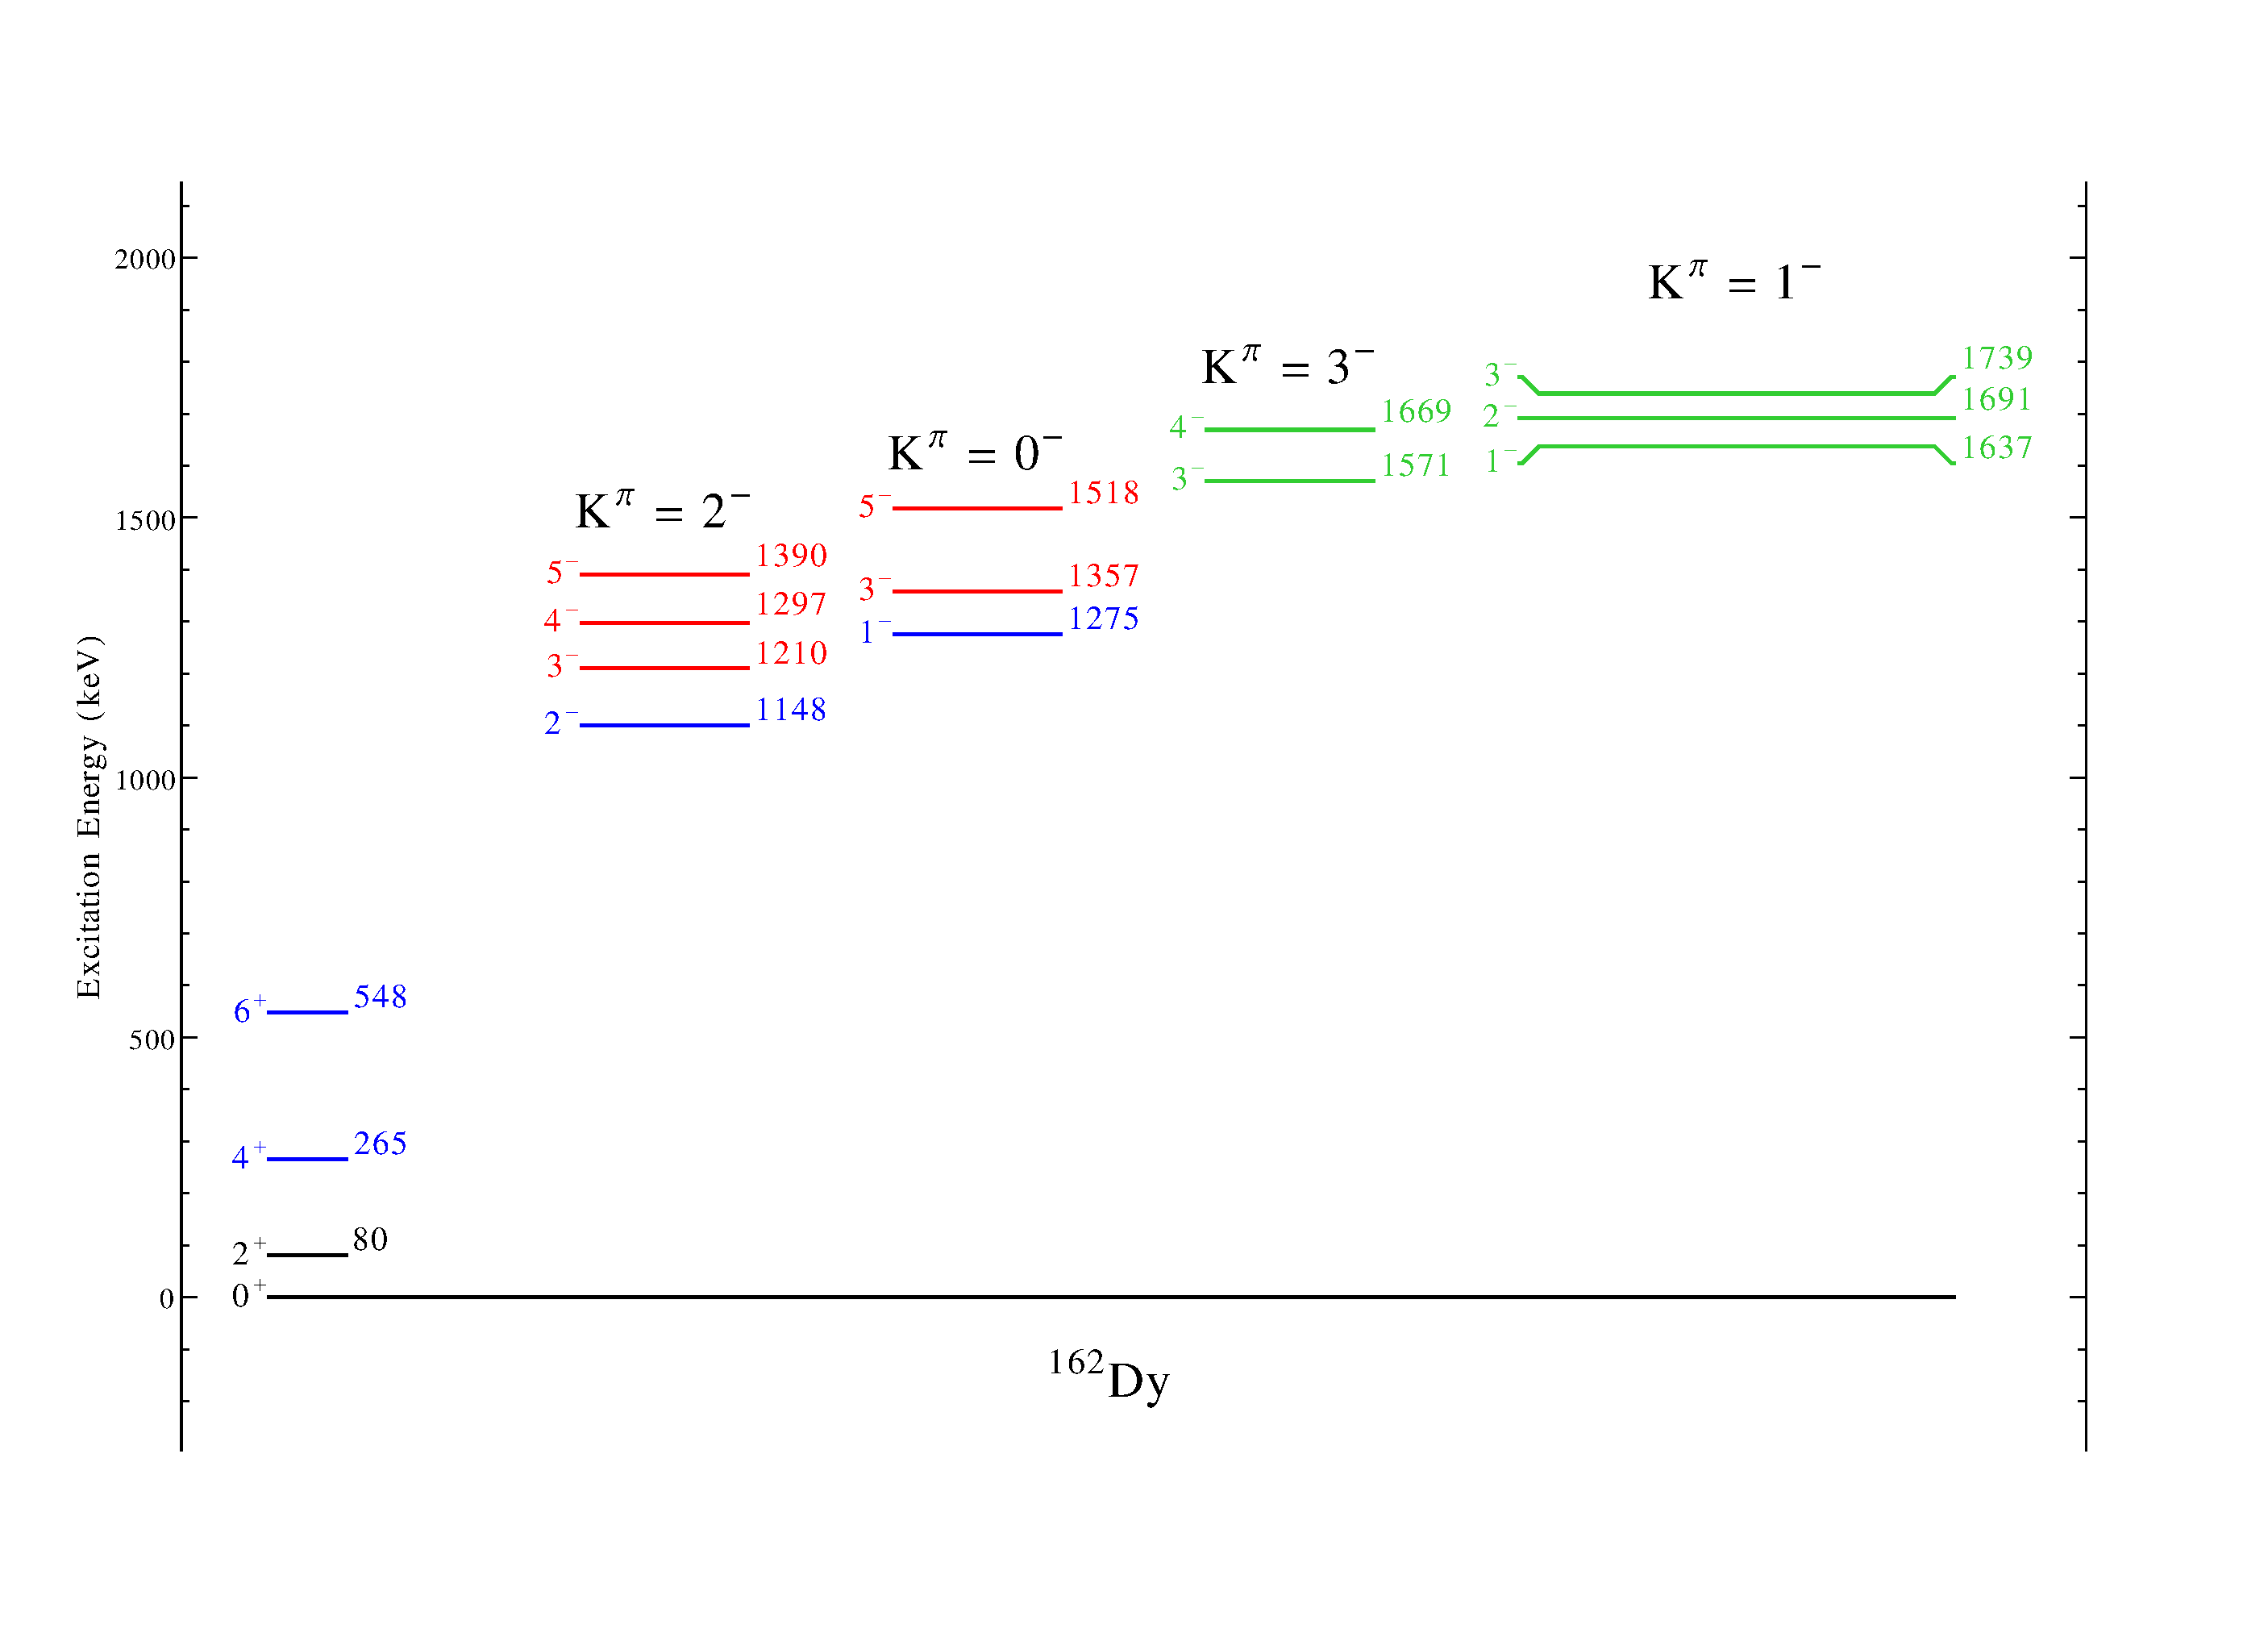
\includegraphics[width=0.95\textwidth]{figures/162Dy_LLoct.pdf}
\caption{Lowest-lying negative parity bands in $^{162}$Dy with reliable lifetimes measured in our experiments in red, existing literature values in blue, and unreliable lifetimes measured in green (color online). \label{fig:162Dy_LLoct}}
\end{center}
\end{figure}

A total of 10 well-convergent level lifetimes were measured (8 of which are new) for three negative parity bands in $^{162}$Dy. All observed transitions from negative parity bands can be seen in Figure \ref{fig:162Dy_negparity_202}, with corresponding transition strengths from Table \ref{tab:162Dy_negparity_202}. Absolute intensities of $\gamma$-decays reported in this work can be seen in Table \ref{tab:162Dy_neg202_intensities}. The traditional picture of octupole collectivity in well-deformed nuclei exists with the initial, lowest-lying and quartet of states of K$^\pi$=0$^-$, 1$^-$, 2$^-$, \& 3$^-$. However, the current ordering of negative parity bands in $^{162}$Dy is difficult (read: impossible) to predict with modern models \cite{Aprahamian200642}. We have measured lifetimes for two bands of this lowest-lying set of states in $^{162}$Dy, where we provide individual discussion on our measurements.


% \begin{table}[h!]
\begin{landscape}
\begin{center}
\begin{longtable}{llcccllc}
\caption{NEGATIVE PARITY BANDS (K$^\pi$=2$^-$,0$^-$,2$^-_2$): $^{162}$DY \label{tab:162Dy_negparity_202}}\\

% \makebox[\textwidth]{
% \begin{tabular}{llcccllc}
E$_{level}$ (keV) & E$_\gamma$ (keV) & J$^\pi_{K^\pi_i}$ & J$^\pi_{K^\pi_f}$   & F($\tau$)$_{av}$ & $\tau$ (fs)                     & BR        & B(E1) (mW.u.)\\ \hline \hline \endfirsthead
\caption[]{NEGATIVE PARITY BANDS (K$^\pi$=2$^-$,0$^-$,2$^-_2$): $^{162}$DY}{Continued}\\

% \makebox[\textwidth]{
% \begin{tabular}{llcccllc}
E$_{level}$ (keV) & E$_\gamma$ (keV) & J$^\pi_{K^\pi_i}$ & J$^\pi_{K^\pi_f}$   & F($\tau$)$_{av}$ & $\tau$ (fs)                     & BR        & B(E1) (mW.u.)\\ \hline \hline \endhead
 1148.20(20) &  260.16(50)               & 2$^-_{2^-_1}$      & 2$^+_{2^+_1}$ &0.074$\pm$0.058& 2100$^{+7200}_{-950}$ $^{[\varsigma]}$          &1.000                 & 8.9$^{+7.3}_{-6.9}$  \\ 
 1210.05(18) &  247.27(55)$^{[\oslash]}$ & 3$^-_{2^-_1}$      & 3$^+_{2^+_1}$ &0.052$\pm$0.030& 3100$^{+3700}_{-1200}$ $^{[\varsigma]}$         &0.056(2)              & 0.2$^{+0.2}_{-0.1}$ \\
             &  322.05(51)$^{[\oslash]}$ & 3$^-_{2^-_1}$      & 2$^+_{2^+_1}$ &&                                                            &0.083(2)              & 0.2$^{+0.1}_{-0.1}$ \\
             &  944.48(50)               & 3$^-_{2^-_1}$      & 4$^+_{0^+_1}$ &&                                                            &0.310(4)              & 0.04$^{+0.03}_{-0.02}$  \\
             & 1129.46(50)$^{[\oslash]}$ & 3$^-_{2^-_1}$      & 2$^+_{0^+_1}$ &&                                                            &0.552(4)              & 0.04$^{+0.03}_{-0.02}$  \\ 
 1297.06(27) &  236.09(60)$^{[\oslash]}$ & 4$^-_{2^-_1}$      & 4$^+_{2^+_1}$ &0.103$\pm$0.049& 1400$^{+1500}_{-350}$ $^{[\varsigma]}$          &0.150(5)              & 2.7$^{+0.9}_{-1.4}$    \\
             &  334.15(50)               & 4$^-_{2^-_1}$      & 3$^+_{2^+_1}$ &&                                                            &0.850(5)              & 5.3$^{+1.8}_{-2.8}$   \\ 
 1390.52(35) & 1124.88(88)               & 5$^-_{2^-_1}$      & 4$^+_{0^+_1}$ &0.090$\pm$0.082& $>$920 $^{[\varsigma]}$                         &1.000                 & $<$0.3               \\ \hline
 1275.81(24) & 1195.10(50)               & 1$^-_{0^-_1}$      & 2$^+_{0^+_1}$ &0.568$\pm$0.028& 120$^{+10}_{-10}$ $^{[\vartheta]}$             & 0.605(6)             & 1.0$^{+0.1}_{-0.1}$ \\
             & 1275.82(53)               & 1$^-_{0^-_1}$      & 0$^+_{0^+_1}$ &&                                                            & 0.395(6)             & 0.5$^{+0.1}_{-0.1}$ \\ 
 1358.00(30) & 1092.27(71)               & 3$^-_{0^-_1}$      & 4$^+_{0^+_1}$ &0.612$\pm$0.043& 100$^{+20}_{-20}$ $^{[\vartheta]}$             & 0.429(9)             & 1.1$^{+0.3}_{-0.2}$ \\ 
             & 1277.33(58)               & 3$^-_{0^-_1}$      & 2$^+_{0^+_1}$ &&                                                            & 0.571(9)             & 0.9$^{+0.2}_{-0.2}$  \\ 
 1518.47(29)&   970.01(55)               & 5$^-_{0^-_1}$ & 6$^+_{0^+_1}$      &0.372$\pm$0.041& 270$^{+80}_{-50}$ $^{[\varsigma]}$              &0.294(7)              & 0.4$^{+0.1}_{-0.1}$         \\
            &  1252.74(51)               & 5$^-_{0^-_1}$ & 4$^+_{0^+_1}$      &&                                                            &0.706(7)              & 0.4$^{+0.1}_{-0.1}$         \\ \hline
 1863.85(26)&   900.90(55)               & 2$^-_{2^-_2}$ & 3$^+_{2^+_1}$      &0.297$\pm$0.035& 420$^{+120}_{-80}$ $^{[\varsigma]}$             &0.251(5)              & 0.3$^{+0.1}_{-0.1}$        \\
            &   975.65(50)               & 2$^-_{2^-_2}$ & 2$^+_{2^+_1}$      &&                                                            &0.749(5)              & 0.6$^{+0.1}_{-0.1}$        \\ 
 1910.50(26)&   947.51(56)               & 3$^-_{2^-_2}$ & 3$^+_{2^+_1}$      &0.250$\pm$0.063& 550$^{+260}_{-180}$ $^{[\varsigma]}$            &0.552(8)              & 0.4$^{+0.2}_{-0.1}$         \\
            &  1022.33(53)               & 3$^-_{2^-_2}$ & 2$^+_{2^+_1}$      &&                                                            &0.448(8)              & 0.3$^{+0.1}_{-0.1}$        \\ 
 1972.99(66)&   912.09(50)               & 4$^-_{2^-_2}$ & 4$^+_{2^+_\gamma}$ &0.205$\pm$0.053& 780$^{+280}_{-210}$    $^{[\varpi]}$       &0.246(13)             & 0.1$^{+0.1}_{-0.1}$\\            
            &  1010.19(50)               & 4$^-_{2^-_2}$ & 3$^+_{2^+_\gamma}$ &&                                                            &0.754(13)             & 0.3$^{+0.1}_{-0.1}$\\ \hline  
% \end{tabular}
% }
\\
\end{longtable}
\end{center}
Lifetimes of negative parity bands (2$^-$, 0$^-$, 2$^-_2$) in $^{162}$Dy, with experimentally deduced B(E1) in mW.u.\\
{\small $^{[\oslash]}$: $\gamma$ ray not used in F($\tau$) calculation (F($\tau$)$<$0).}\\
{\small $^{[\vartheta]}$: F($\tau$) extracted from E$_n$=1.6~MeV angular distributions},
{\small $^{[\varsigma]}$: F($\tau$) extracted from E$_n$=2.2~MeV angular distributions},
{\small $^{[\varpi]}$: F($\tau$) extracted from E$_n$=3.1~MeV angular distributions}\\
{\small $^{[\dagger]}$: Lifetime not reliable (F($\tau$) consistent with zero within 1$\sigma$)}\\
{\small 1~mW.u.=1.91 e$^2$b}
% \end{table}
\end{landscape}


We are immediately presented with some of the limitations of DSAM with our measurement of the lifetime of the bandhead of the K$^\pi$=2$^-$ band. Firstly, $\gamma$-ray energies can be heavily attenuated in the physical size of the near-molar-weight target; while we correct for this $\gamma$ absorption in the peak area/intensity, lifetimes from the Doppler shift of $\gamma$-rays sub-500~keV are difficult to extract, as F($\tau$) can be within 1 or 2$\sigma$ of 0. Normally, DSAM measurements are taken at the lowest possible bombarding neutron energy, but due to this attenuation of low-energy $\gamma$ rays, a more precise measurement of the lifetimes in this band are taken from the 2.2~MeV bombarding neutron dataset. While we expect a natural inflation of the lifetimes because of this choice of neutron energy, the vast majority of observed transitions displayed negative (or consistent with zero within 1$\sigma$ uncertainty) F($\tau$) values. This justification is supported by Figure \ref{fig:260_DSAM_EXF}, which shows all excitation functions for $\gamma$ rays that both de-excite this band and contribute to the lifetime; take note that the gain in statistics by a factor of $\sim$2 by increasing the neutron energy, where we are exempt from higher-lying decays acting as a contaminant (see the trajectories as the neutron energy increases to 3.1~MeV). Extraction of the lifetime for the bandhead at 2100$^{+7200}_{-950}$~fs involves the measurement of a 260~keV $\gamma$ ray, shown in Figure \ref{fig:260_DSAM_EXF}, and does not agree with the literature value of 303~ps \cite{PhysRev.166.1227}, as the shallow F($\tau$) is just over 1$\sigma$ away from 0, making this lifetime partially unreliable. We do not observe the other decay channel to the 3$^+$ member of the $\gamma$-band, as that decay energy is 185~keV, directly on top of our strongest line in our spectra, the ground state 4$^+\rightarrow$2$^+$ transition. With no higher energy decays observed to the ground state, we report this measurement of the bandhead's lifetime, but it should be taken as a tentative, cautious measurement, given the very large discrepancy from literature. However, we regain good lifetime resolution on the measurement of the 3$^-$ and 4$^-$ bandmembers; the former state's lifetime of 3100$^{+3700}_{-1200}$~fs comes from the 944~keV $\gamma$ ray, where the other exit channels have either a negative F($\tau$) value. 

\begin{figure}[h!]
\begin{center}
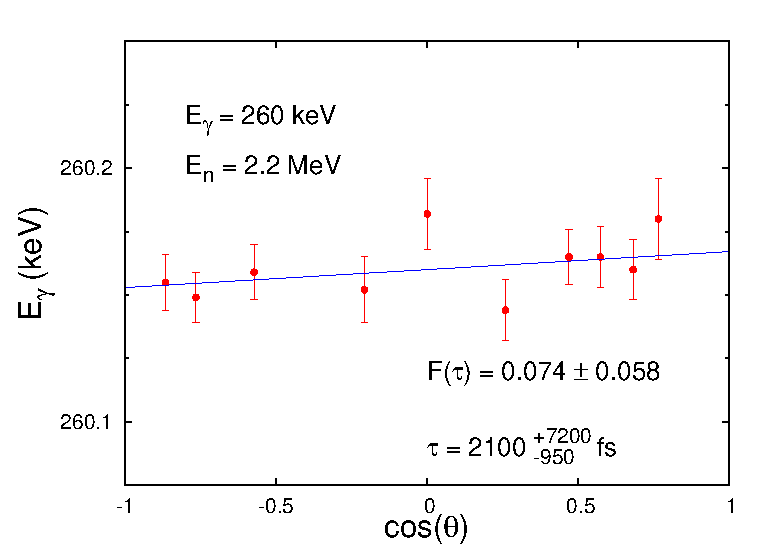
\includegraphics[width=0.49\textwidth]{figures/260_DSAM.eps}
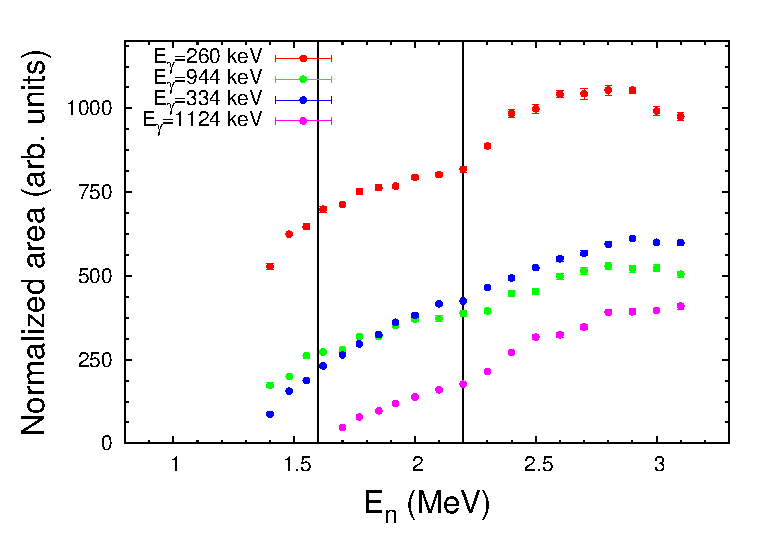
\includegraphics[width=0.49\textwidth]{figures/260_ExF.eps}
\caption{E$_\gamma$=260~keV $\gamma$ ray (from the E$_{\rm x}$=1148~keV level) Doppler shift and excitation functions for decays from the first 2$^-$ band (color online). The vertical black lines highlight our justification for using a slightly higher bombarding neutron energy, for the sake of better statistics, without the potential for contaminant decay channels from other states. \label{fig:260_DSAM_EXF}}
\end{center}
\end{figure}

We have measured lifetimes for the 3 lowest-lying members of the 0$^-$ band, currently assigned as the single octupole vibration in $^{162}$Dy from the clearly collective literature B(E3;3$^-\rightarrow$0$^+_{gs}$) measurements ranging from 1.4-4.7~W.u. \cite{KORTEN_1993,OEHLBERG_BE3}. The deduced lifetime from the direct B(E1)$\uparrow$ measurement in \cite{Zilges_K0dipole} of the bandhead of the K$^\pi$=0$^-$ band has been called into question by the NDS evaluator, with the distinct comment that the $\gamma$-branches of E1 radiation depopulating the state differs drastically from the adopted values. We are confident in our lifetime measurement from the extremely well-defined Doppler energy-shifts of the two de-excitations from this E$_{\rm x}$=1275~keV level (shown in Figure \ref{fig:1275_DSAM_EXF}). The 5$^-$ state at 1518~keV is below the threshold to be populated by E$_n$=1.6~MeV neutrons, the de-excitations are not observed until the E$_n$=2.2~MeV dataset; this implies that the resulting lifetime will be inflated, as F($\tau$) is directly related to the bombarding neutron energy.

The final set of lifetime measurements of negative parity states is the second K$^\pi$=2$^-$ band. Two $\gamma$-ray placements from \cite{Aprahamian200642} are made into the bandhead of this 2$^-$ band, the 900 and 975~keV transitions, both showing a well-behaved Doppler shift to yield a level lifetime of 420$^{+120}_{-80}$~fs.  We have also placed two $\gamma$-ray transitions from the E$_{\rm x}$=1974~keV 4$^-$ state \cite{BERZINS1995413}, a 912~kev and a 1010~keV decay to the $\gamma$-vibrational band. Confirmation of the placement of these de-excitations is made with the measurement of the excitation functions, shown in Figure \ref{fig:1974_DSAM_EXF}; these $\gamma$-rays were also observed in \cite{Aprahamian200642}, but were unplaced in their level scheme. Our absolute intensities are in reasonable agreement with the literature values in \cite{Aprahamian200642,BERZINS1995413}, further justifying their correct placement in the level scheme. 

\begin{figure}[h!]
\begin{center}
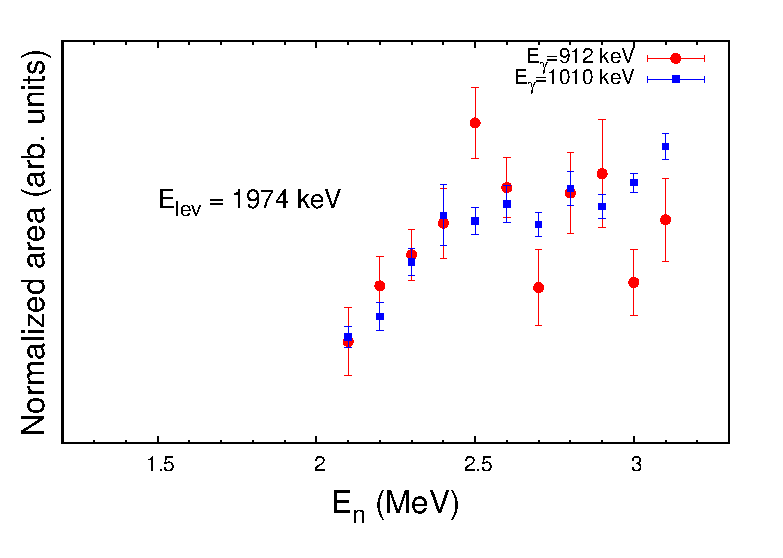
\includegraphics[width=0.75\textwidth]{figures/1974_ExF.eps}\\
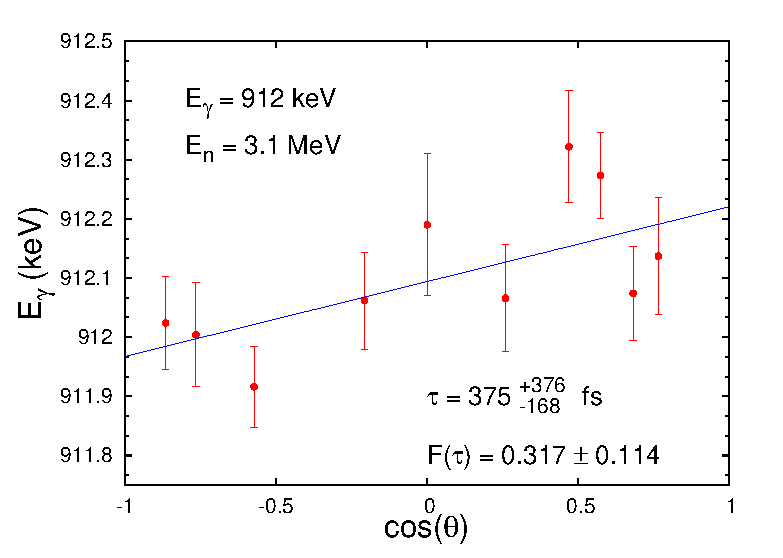
\includegraphics[width=0.49\textwidth]{figures/912_DSAM.eps}
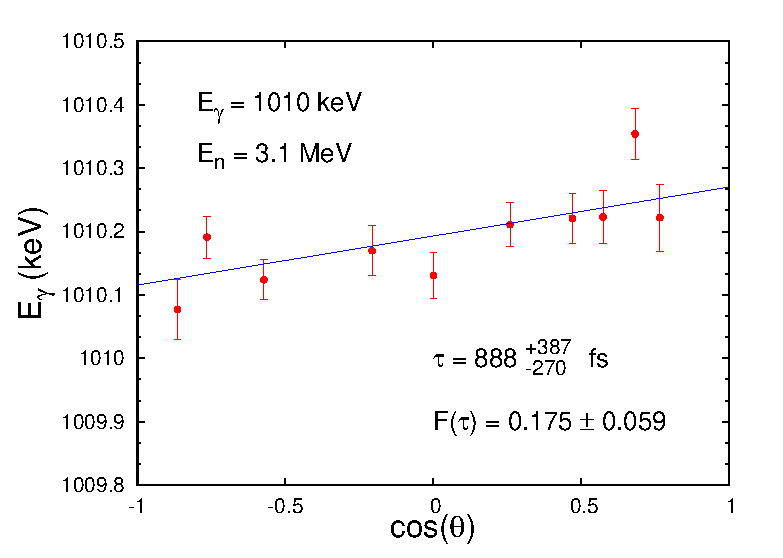
\includegraphics[width=0.49\textwidth]{figures/1010_DSAM.eps}

\caption{E$_\gamma$=912 \& 1010~keV (de-excitations from the E$_{\rm x}$=1974~keV level) Doppler shifts and excitation functions (color online). The excitation function (in blue) for the 1010~keV $\gamma$ ray is scaled by a factor of 0.33 to normalize to the branching ratio of the level. \label{fig:1974_DSAM_EXF}}
\end{center}
\end{figure}

\subsection{Lifetimes of Other Negative Parity Bands (K$^\pi$=5$^-$, 3$^-$, 1$^-$ and 3$^-_2$)}

Our discrepancy in lifetime measurement with respect to the literature value for the K$^\pi$=5$^-$ bandhead is striking, much like the case for the E$_{\rm x}$=1148~keV level, yet we repeat the same assertions made in the previous section. The two de-exciting $\gamma$-rays exhibit a rather unambiguous placement in the level scheme from our measurement of the excitation function (both E$_\gamma$=937 \& 1220~keV $\gamma$ rays match qualitative shape and have the same threshold, consistent with a 5$^-$ state at 1485~keV), and show well-defined Doppler energy-shifts that correspond to a lifetime of 450~fs, compared to the literature value of 1.92~ns \cite{Honig_5minus1969}. We contest this lifetime measurement via delayed-coincidence from the $\beta$-decay of $^{162m}$Ho, from our unambiguous placement of de-exciting $\gamma$ rays in the level scheme, accurate branching ratios in comparison to literature intensities, and well-behaved DSAM shifts. In scrutinization of the literature, it is found that the 1.92~ns lifetime measurement by \cite{Honig_5minus1969} is explicitly placed for the nearby 1490~keV state, and very little discussion is made on the delayed-coincidence measurements made in \cite{CHARVET_162Dy5minus}. It is not entirely unreasonable that the measured lifetime in \cite{Honig_5minus1969,CHARVET_162Dy5minus} are instead seeing this nearby state at 1490~keV. This 7$^+$ state de-excites via a very similar energy (940~keV versus 937~keV) $\gamma$ ray, and is populated via first-forbidden Fermi-type $\beta$-decay, in contrast to the preferred Gamov-Teller decay to the 5$^-$ at 1485~keV. 

\begin{figure}[h!]
\begin{center}
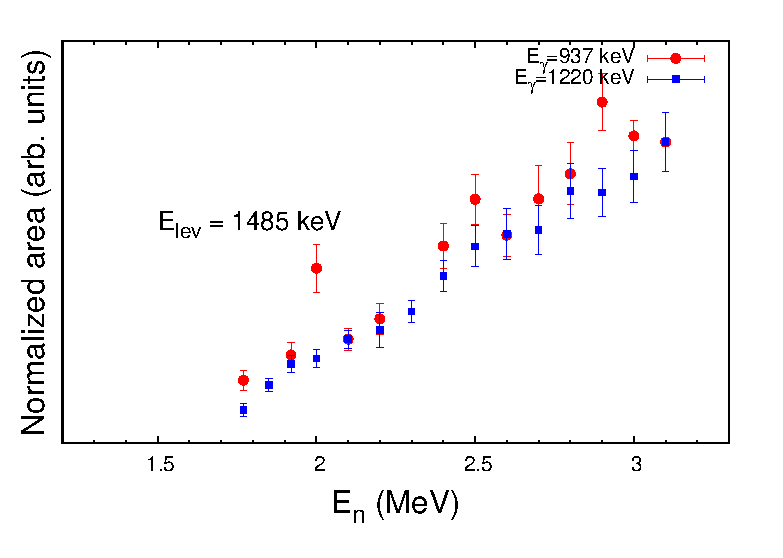
\includegraphics[width=0.75\textwidth]{figures/937_ExF.eps}\\
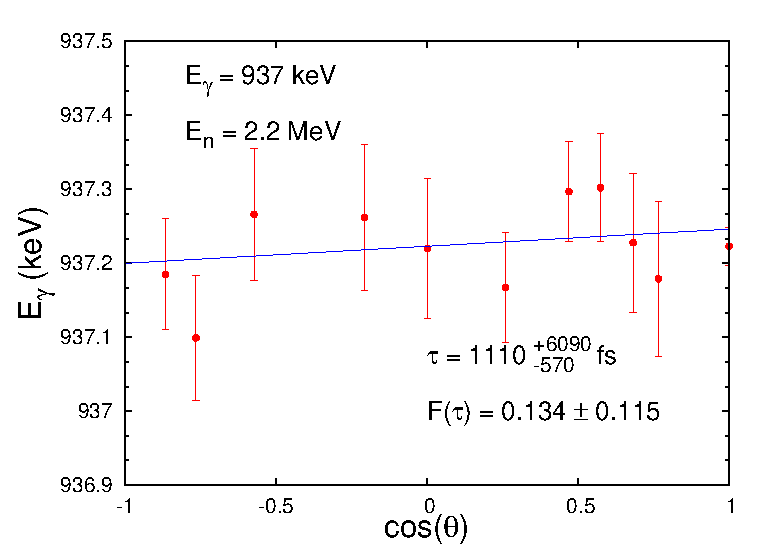
\includegraphics[width=0.49\textwidth]{figures/937_DSAM.eps}
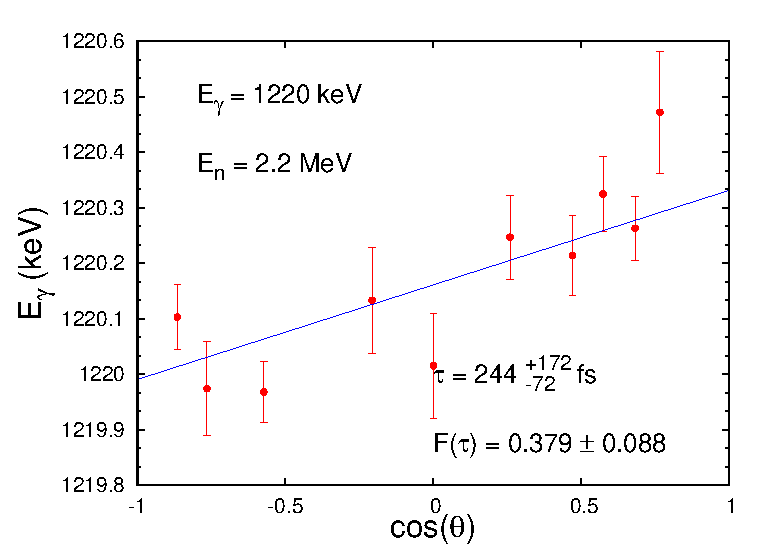
\includegraphics[width=0.49\textwidth]{figures/1220_DSAM.eps}
\caption{E$_\gamma$=937 \& 1220~keV (de-excitations from the E$_{\rm x}$=1485~keV level) Doppler shifts and overlaid excitation functions (color online). The excitation function (in blue) for the 1220~keV $\gamma$ ray is scaled by a factor of 0.291. \label{fig:1485_DSAM_EXF}}
\end{center}
\end{figure}


Absolute intensities from $\gamma$ rays depopulating the K$^\pi$=3$^-$ band at 1570~keV show an obvious preference to the previously established 0$^-$ octupole band \cite{Aprahamian200642} in the literature, where we do not observe the full 3$^-\rightarrow$\textit{g.s.} transitions due to the low branching ratios listed. Shallow shifts in the DSAM fitting only gives a lower limit to the lifetime of the 3$^-$ bandhead of $>$3050~fs, where, in contrast, we get good lifetime resolution on the 4$^-$ member. That being said, we yet again encounter some of the limitations behind the Doppler Shift Attenuation Method, in that lower energy $\gamma$ rays ($<$500~keV) are easily attenuated by the sample size and may not exhibit reliable energy shifts. Further investigation of this level lifetime with another measurement technique (Coulomb excitation, `plunger' method with RDDM, etc) is desired to more confidently understand the transition probabilities here, as the lifetimes measured in our campaign of experiments seem to be fairly unreliable. 


The K$^\pi$=1$^-$ band at 1637~keV provides some of the least consistent and reliable results from our experimental campaign to measure lifetimes in $^{162}$Dy. Starting with the bandhead, the only $\gamma$ ray to attribute to the lifetime measurement is the de-excitation of E$_\gamma$=1637~keV. The questionability of this $\gamma$-ray placement is an issue, in that (n,$\gamma$) reactions by \cite{Aprahamian200642} do not observe it, yet other (n,n$^\prime\gamma$) experiments do. Nevertheless, the other two observed decays cannot be used because the 427~keV line is coincident with a background line, and as such, the extracted F($\tau$) is not reliable; the 489~keV $\gamma$ provides an alternate discussion on its exclusion from the level lifetime. First, the relative intensity of the radiation does not fall in line with the other de-excitations according to the literature, and second, the extracted F($\tau$) from the 427~keV line varies wildly (by more than 2$\sigma$) from the 1637~keV line, and lastly, the excitation function(s) (Figure \ref{fig:162Dy_ExF1637}) for de-excitations out of the bandhead show an inconclusively similar pattern, qualitatively. These reasons are indicative of a bad placement of this decay in the level scheme, and is indicated by parentheses in Table \ref{tab:162Dy_negparity_5313}. Further proof of the 489~keV $\gamma$ ray being a contaminant can be seen in the nonconvergence of a multipole mixing fraction (ranging from 33-91\% E2, with a large $\chi^2$ value on the angular distribution).

The 2$^-$ member of the band also yields some less than stellar resolution on the nuclear lifetime. With two decays observed at intermediate energies (but still below 1~MeV), we are only able to rely on the 728~keV $\gamma$ ray to measure the lifetime, as the 416~keV decay lies on top of a background. The resulting lifetime limit of $>$1000~fs extracted from the Doppler Shift is not reliable, with F($\tau$) being consistent with zero within 1$\sigma$ uncertainty. Since the 416~keV $\gamma$ ray is coincident with a background, a reliable multipole mixing fraction cannot be extracted from the angular distributions, as we do not know the distribution of the background as a function of angle. 

The 3$^-$ member offers a slight tangent from the echoed rhetoric of lifetime measurements in the 1$^-$ band, but still does not provide well-defined DSAM lifetimes. The extracted average level F($\tau$) value is just over 1$\sigma$ deviant from 0, giving both a) a borderline unreliable lifetime extraction, and b) an extremely low magnitude lower limit of $>$740~fs. In this sea of delinquent behavior, the branching ratios for the 3$^-$ state of the 1$^-$ band agree well with literature \cite{Aprahamian200642}, but the multipole mixing fraction for the 529~keV $\gamma$ is deviant from literature ($\sim$50\% mixed, vs $>$99\% M1 in literature). %Again, the resulting B($\pi\ell$) strengths for decays out of the 3$^-$ state are vast upper limits from our experiments. 


\begin{figure}[h!]
\begin{center}
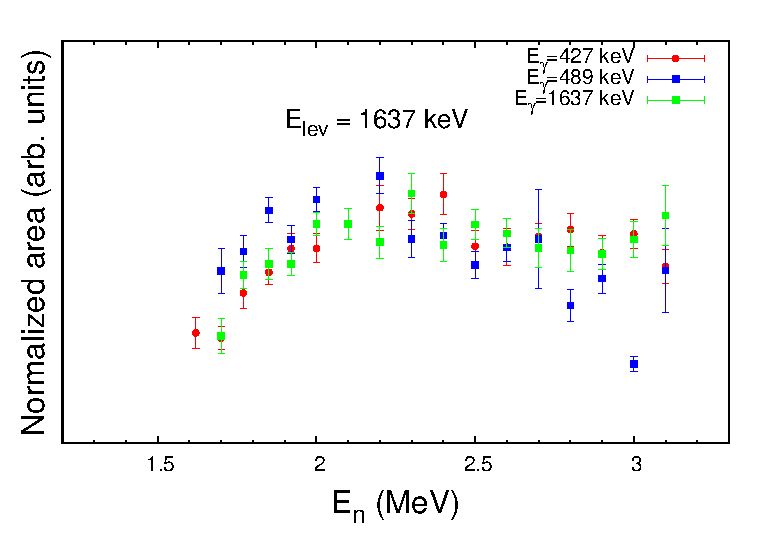
\includegraphics[width=0.97\textwidth]{figures/162Dy_1minus_ExF.eps}
\end{center}
\caption{Excitation functions for the decays leaving the E$_{\rm x}$=1637~keV state. Note the differing population threshold energies for each $\gamma$-ray. (color online)\label{fig:162Dy_ExF1637}}
\end{figure}

%3-_2
F($\tau$) values for the bandhead of the second K$^\pi$=3$^-$ band at 1766~keV fail to display any definite shift in energy, in fact, having a negative (completely unphysical) value with a very large error. The unreliable lifetime reported in this work is simply the lower limit where F($\tau$) is the most positive, at a value of 0.044, but this extracted lifetime of 3400~fs should not be taken with any amount of confidence. The same can be said about the 4$^-$ member at 1826~keV: the extracted F($\tau$) is \textit{very} consistent with zero, as the only available transition to $\gamma$-band at 863~keV transition energy gives an appreciably nonzero shift (though not by much). Again, the lower limit of the lifetime is taken at the very edge of what F($\tau$) can be (at a value of 2400~fs).The statistical model employed ({\tt CINDY} \cite{SHELDON197399}) to calculate multipole mixing fractions was able to converge on a value for the mixing ratio from the 556~keV $\gamma$ ray's angular distribution, however.

% \begin{table}[h!]
\begin{landscape}
\begin{center}
\begin{longtable}{clllllllcc}
\caption{NEGATIVE PARITY BANDS (K$^\pi$=5$^-$,3$^-$,1$^-$,3$^-_2$): $^{162}$DY \label{tab:162Dy_negparity_5313}}\\
% \resizebox{1.15\linewidth}{!}{
% \begin{tabular}{clllllllcc}
E$_{lev}$ (keV) & E$_\gamma$ (keV)        & J$_i$              & J$_f$        & F($\tau$)$_{av}$ & $\tau$ (fs)                           & BR        & $\pi\ell$ & $\delta_{mix}$      & B($\pi\ell$) \\ \hline\hline \endfirsthead
\caption[]{NEGATIVE PARITY BANDS (K$^\pi$=5$^-$,3$^-$,1$^-$,3$^-_2$): $^{162}$DY}{Continued}\\
% \resizebox{1.15\linewidth}{!}{
% \begin{tabular}{clllllllcc}
E$_{lev}$ (keV) & E$_\gamma$ (keV)        & J$_i$              & J$_f$        & F($\tau$)$_{av}$ & $\tau$ (fs)                           & BR        & $\pi\ell$ & $\delta_{mix}$      & B($\pi\ell$) \\ \hline\hline \endhead
 1485.79(29)&   937.23(56)               & 5$^-_{5^-_1}$ & 6$^+_{0^+_1}$      &0.310$\pm$0.070& 400$^{+210}_{-140}$ $^{[\varsigma]}$            &0.257(10)            & E1    &                                      & 0.3$^{+0.1}_{-0.1}$         \\
            &  1220.16(56)               & 5$^-_{5^-_1}$ & 4$^+_{0^+_1}$      &&                                                            &0.743(10)            & E1    &                                      & 0.3$^{+0.2}_{-0.1}$         \\ \hline
 1570.82(27)&   212.89(51)$^{[\oslash]}$ & 3$^-_{3^-_1}$ & 3$^-_{0^-_1}$      &0.015$\pm$0.036& $>$3200$^{[\varpi,\dagger]}$               &0.348(9)             & E2/M1 &-0.48$^{+0.13}_{-0.16}$ $^{[\varsigma]}$  & $<$720         \\
            &   295.23(50)               & 3$^-_{3^-_1}$ & 1$^-_{0^-_1}$      &&                                                            &0.652(9)             & E2    &                                      & $<$1400         \\ 
 1669.26(38)&   311.27(50)               & 4$^-_{3^-_1}$ & 3$^-_{0^-_1}$      &0.289$\pm$0.116& 440$^{+450}_{-210}$ $^{[\varsigma]}$            &1.000                & E2/M1 & -6.9$^{+1.6}_{-2.2}$ $^{[\varsigma]}$    & 12000$^{+6000}_{-11000}$ $^{[\dagger]}$        \\ \hline 
 1637.52(20)&   427.62(52)$^{[\otimes]}$ & 1$^-_{1^-_1}$ & 3$^-_{2^-_1}$      &0.081$\pm$0.052& 2000$^{+3500}_{-800}$ $^{[\varpi]}$        &0.418(8) $^{[\star]}$& E2                                 && 230$^{+150}_{-140}$                    \\
            &  (489.05(56)$^{[\oslash]}$)& 1$^-_{1^-_1}$ & 2$^-_{2^-_1}$      &&                                                            &0.157(9)             & E2/M1 &  0.7$<\delta<$3.2 $^{[\varsigma]}$       & 40$^{+25}_{-27}$           \\
            &  1637.68(55)               & 1$^-_{1^-_1}$ & 0$^+_{0^+_1}$      &&                                                            &0.425(9)             & E1    &                                      & 0.02$^{+0.01}_{-0.01}$              \\ 
 1691.72(23)&   416.00(51)$^{[\otimes]}$ & 2$^-_{1^-_1}$ & 1$^-_{0^-_1}$      &0.060$\pm$0.087& $>$1000 $^{[\varsigma,\dagger]}$                &0.483(8)$^{[\star]}$ & E2/M1 & ---$^{[\ddagger]}$                   & $<$630  \\
            &   728.50(51)               & 2$^-_{1^-_1}$ & 3$^+_{2^+_1}$      &&                                                            &0.517(8)             & E1    &                                      & $<$0.4  \\  
 1739.02(21)&   529.06(51)$^{[\oslash]}$ & 3$^-_{1^-_1}$ & 3$^-_{2^-_1}$      &0.107$\pm$0.098& $>$740 $^{[\varsigma]}$                         &0.375(6)             & E2/M1 & 1.4$^{+0.2}_{-0.2}$ $^{[\varsigma]}$     & $<$130 \\
            &   590.74(54)               & 3$^-_{1^-_1}$ & 2$^-_{2^-_1}$      &&                                                            &0.139(5)             & E2/M1 & 1.2$^{+0.5}_{-0.3}$ $^{[\varsigma]}$     & $<$24 \\
            &   678.12(53)               & 3$^-_{1^-_1}$ & 4$^+_{2^+_1}$      &&                                                            &0.238(5)             & E1    &                                      & $<$0.3 \\
            &  1473.36(53)$^{[\oslash]}$ & 3$^-_{1^-_1}$ & 4$^+_{0^+_1}$      &&                                                            &0.248(5)             & E1    &                                      & $<$0.03 \\ \hline
 1766.56(26)&   556.67(59)$^{[\oslash]}$ & 3$^-_{3^-_2}$ & 3$^-_{2^-_1}$      &-0.061$\pm$0.105& $>$3400 $^{[\varsigma,\dagger]}$               &0.310(12)            & E2/M1 & -0.54$^{+0.16}_{-0.21}$ $^{[\varsigma]}$ & $<$6 $^{[\dagger]}$    \\
            &   878.21(55)$^{[\oslash]}$ & 3$^-_{3^-_2}$ & 2$^+_{2^+_1}$      &&                                                            &0.690(12)            & E1    &                                      & $<$0.1 $^{[\dagger]}$     \\ 
 1826.64(28)&   643.99(54)$^{[\otimes]}$ & 4$^-_{3^-_2}$ & 5$^+_{2^+_1}$      &0.002$\pm$0.066& $>$2400 $^{[\varpi,\dagger]}$              &0.265(9) $^{[\star]}$& E1     &                                     & $<$0.1       \\
            &   863.84(54)               & 4$^-_{3^-_2}$ & 3$^+_{2^+_1}$      &&                                                            &0.735(9)             & E1     &                                     & $<$0.2      \\ \hline


% \end{tabular}
% }    
\end{longtable}
\end{center}
Lifetimes of 5$^-$, 3$^-$, 1$^-$, and second 3$^-$ bands in $^{162}$Dy, with experimentally deduced B(E1) in mW.u. and B(E2) in W.u.
{\small $^{[\oslash]}$: $\gamma$ ray not used in F($\tau$) calculation (F($\tau$)$<$0).}\\
{\small $^{[\vartheta]}$: F($\tau$) extracted from E$_n$=1.6~MeV angular distributions},
{\small $^{[\varsigma]}$: F($\tau$) extracted from E$_n$=2.2~MeV angular distributions},
{\small $^{[\varpi]}$: F($\tau$) extracted from E$_n$=3.1~MeV angular distributions}\\
{\small $^{[\dagger]}$: Lifetime not reliable (F($\tau$) consistent with zero within 1$\sigma$),}
{\small $^{[\otimes]}$: $\gamma$ ray not used in F($\tau$) calculation (coincident with background), $^{[\star]}$: branching ratio not reliable due to background contamination.}
{\small 1~W.u.(E2)=5.25E-7~e$^2$b$^2$, 1~mW.u.(E1)=1.91 e$^2$b}

\end{landscape}
% \end{table}

\subsection{Lifetimes of K$^\pi$=1$^+$ Band and Members of M1 Scissors}
Our measurement of lifetimes in the 1$^+$ band can be seen in Table \ref{tab:162Dy_1plusminus}, where we have two good F($\tau$) shifts, and two unreliable measurements of the lifetime of states. The bandhead is the first of the unreliable lifetimes measured. Here, the only $\gamma$ decay that contributes to the calculation of a level lifetime is the 857~keV $\gamma$ ray, but the energy shift is consistent with zero within 1$\sigma$ uncertainty. While this is not a low-energy decay that would be more susceptible to attenuation in the sample, it \textit{may} be a contaminant, as the angular distribution does not yield a reliable mixing ratio for the decay. 

The 2$^+$ member of this band echoes a similar story; one de-excitation is not used in the determination of the nuclear lifetime, as the F($\tau$) measured is negative. However, unlike the bandhead, this $\gamma$-ray angular distribution that is excluded (1701~keV) converges on a good, reliable value for E2/M1 mixing, at just under 50\% mixing. That being said, the extracted lifetime is still not reliable, since F($\tau$) for this level is negative. 

The decays to both the ground state 4$^+$ and the $\gamma$-band 4$^+$ are used to extract the lifetime of 1400$^{+4500}_{-1000}$~fs for this 3$^+$ state at 1840~keV. To round out the K$^\pi$=1$^+$ band, the 4$^+$ state at 1951~keV offers good lifetime resolution, similar to the 3$^+$ state.


% \begin{table}[h!]
\begin{landscape}
\begin{center}
\begin{longtable}{clcccllccc}
\caption{K$^\pi$=1$^\pm$ AND M1 SCISSORS MODE: $^{162}$DY \label{tab:162Dy_1plusminus}}\\

% \resizebox{1.15\linewidth}{!}{
% \begin{tabular}{clcccllccc}
E$_{lev}$ (keV) & E$_\gamma$ (keV)        & J$_i$              & J$_f$        & F($\tau$)$_{av}$ & $\tau$ (fs)                           & BR        & $\pi\ell$ & $\delta_{mix}$      & B($\pi\ell$) \\
\hline \hline \endfirsthead
\caption[]{K$^\pi$=1$^\pm$ AND M1 SCISSORS MODE: $^{162}$DY}{Continued}\\

% \resizebox{1.15\linewidth}{!}{
% \begin{tabular}{clcccllccc}
E$_{lev}$ (keV) & E$_\gamma$ (keV)        & J$_i$              & J$_f$        & F($\tau$)$_{av}$ & $\tau$ (fs)                           & BR        & $\pi\ell$ & $\delta_{mix}$      & B($\pi\ell$) \\
\hline \hline \endhead
 1745.80(25)&   857.65(50)               & 1$^+_{1^+_1}$ & 2$^+_{2^+_1}$      &0.039$\pm$0.044& $>$1800 $^{[\varsigma,\dagger]}$                &0.538(5)             & E2/M1 & ---$^{[\ddagger]}$                   & $<$0.02 $^{[\dagger]}$        \\
            &  1665.09(51)$^{[\oslash]}$ & 1$^+_{1^+_1}$ & 2$^+_{0^+_1}$      &&                                                            &0.462(5)             & E2/M1 & 0.41$^{+0.27}_{-0.19}$ $^{[\varsigma]}$  & $<$0.04 $^{[\dagger]}$    \\ 
 1782.54(22)&  1701.90(53)$^{[\oslash]}$ & 2$^+_{1^+_1}$ & 2$^+_{0^+_1}$      &0.013$\pm$0.033& $>$3400 $^{[\varpi,\dagger]}$              &0.389(10)            & E2/M1  & 0.33$^{+0.24}_{-0.13}$ $^{[\varsigma]}$ & $<$0.01       \\
            &  1782.63(53)               & 2$^+_{1^+_1}$ & 0$^+_{0^+_1}$      & &                                                           &0.611(10)            & E2     &                                     & $<$0.2       \\ 
 1840.44(21)&   630.51(68)$^{[\oslash]}$ & 3$^+_{1^+_1}$ & 3$^-_{2^-_1}$      &0.104$\pm$0.074& 1400$^{+3500}_{-500}$ $^{[\varsigma]}$          &0.180(10)            & E1    &                                      & 0.2$^{+0.1}_{-0.1}$          \\
            &   779.58(60)               & 3$^+_{1^+_1}$ & 4$^+_{2^+_1}$      &&                                                            &0.283(11)            & E2/M1 & $<$-4.8 $^{[\varsigma]}$                 & 10$^{+8}_{-6}$   \\
            &  1574.82(57)               & 3$^+_{1^+_1}$ & 4$^+_{0^+_1}$      &&                                                            &0.262(12)            & E2/M1 & 4.4$^{+18}_{-2.1}$ $^{[\varsigma]}$      & 0.3$^{+0.2}_{-0.2}$        \\
            &  1759.60(75)$^{[\oslash]}$ & 3$^+_{1^+_1}$ & 2$^+_{0^+_1}$      &&                                                            &0.276(16)            & E2/M1 & 0.21$^{+0.15}_{-0.13}$ $^{[\varsigma]}$  & 0.01$^{+0.01}_{-0.01}$         \\ 
 1951.17(34)&  1685.80(56)               & 4$^+_{1^+_1}$ & 4$^+_{0^+_1}$      &0.071$\pm$0.048& 2300$^{+4500}_{-1000}$ $^{[\varpi]}$       &1.000                & E2/M1  & -0.38$^{+0.14}_{-0.17}$ $^{[\varpi]}$  & 0.1$^{+0.1}_{-0.1}$        \\ \hline
 2395.60(39)& 2395.00(50) & 1$^+_{\Omega}$         & 0$^+_{0^+_1}$ &0.926$\pm$0.061& 14$^{+13}_{-11}$        $^{[\varpi]}$               &1.000                & M1    &                                          & 0.14$^{+0.61}_{-0.08}$    \\ \
 2519.43(36)& 2438.00(51) & 1$^-_{\Omega}$         & 2$^+_{0^+_1}$ &0.595$\pm$0.054& 110$^{+30}_{-20}$       $^{[\varpi]}$               &0.564(27)            & E1    &                                          & 0.1$^{+0.1}_{-0.1}$         \\
            & 2520.27(51) & 1$^-_{\Omega}$         & 0$^+_{0^+_1}$ &&                                                                     &0.436(27)            & E1    &                                          & 0.1$^{+0.1}_{-0.1}$         \\ 
 2537.26(30)& 2537.24(51) & 1$^+_{\Omega}$         & 0$^+_{0^+_1}$ &0.290$\pm$0.049& 460$^{+160}_{-120}$     $^{[\varpi]}$               &1.000                & M1    &                                          & 0.004$^{+0.001}_{-0.001}$   \\ 
 2569.35(22)& 2568.83(51) & 1$^+_{\Omega}$         & 0$^+_{0^+_1}$ &0.653$\pm$0.066& 90$^{+30}_{-20}$        $^{[\varpi]}$               &1.000                & M1    &                                          & 0.021$^{+0.006}_{-0.005}$ \\
 2814.80(33)& 2734.24(55) & 1$^+_{\Omega}$         & 2$^+_{0^+_1}$ &0.442$\pm$0.099& 200$^{+130}_{-60}$      $^{[\varpi]}$               &1.000                & M1    &                                          & 0.008$^{+0.003}_{-0.003}$ \\ \hline

% \end{tabular}
% } \\ 
\end{longtable}
\end{center}  
Lifetimes of 1$^+$ band and 1$^\pm$ members of the isovector M1 scissors mode ([$\Omega$] marker) in $^{162}$Dy, with experimentally deduced B(E1) in mW.u., B(M1) in $\mu_N^2$ and B(E2) in W.u.
{\small $^{[\oslash]}$: $\gamma$ ray not used in F($\tau$) calculation (F($\tau$)$<$0).}\\
{\small $^{[\vartheta]}$: F($\tau$) extracted from E$_n$=1.6~MeV angular distributions},
{\small $^{[\varsigma]}$: F($\tau$) extracted from E$_n$=2.2~MeV angular distributions},
{\small $^{[\varpi]}$: F($\tau$) extracted from E$_n$=3.1~MeV angular distributions}\\
{\small $^{[\dagger]}$: Lifetime not reliable (F($\tau$) consistent with zero within 1$\sigma$)}\\
{\small 1~W.u.(E2)=5.25E-7~e$^2$b$^2$, 1~mW.u.(E1)=1.91 e$^2$b}
% \end{table}
\end{landscape}

\subsection{Lifetimes of States with No K$^\pi$ Assignment}
We direct the reader to the fact that lifetimes above the pairing gap in $^{162}$Dy exhibit very well-behaved and precise lifetime measurements; this is an artifact of the DSAM measurements at UKAL, where, generally, the higher energy $\gamma$ rays that completely de-excite the nucleus fare better in escaping the sample size and displaying a noticeable energy shift than those at lower energy thresholds. Tables \ref{tab:162Dy_miscellaneous} and \ref{tab:162Dy_miscellaneous2} list these `miscellanous' lifetimes for which there is no rotational band assignment for the state. In many of these states, we place liberal limits on the spin/parity, based solely on our measurement of the angular distributions. Because of the tentative spin assignments, multipole mixing fractions extracted from the angular distributions are often unavailable, as the statistical model employed requires known spins and parities to be known.



% \begin{table}[h!]
\begin{landscape}
\begin{center}
\begin{longtable}{clcccllccc}
\caption{OTHER LEVELS (NO K ASSIGNMENT): $^{162}$DY \label{tab:162Dy_miscellaneous}}\\

% \resizebox{1.15\linewidth}{!}{
% \begin{tabular}{clcccllccc}
E$_{lev}$ (keV) & E$_\gamma$ (keV)        & J$_i$              & J$_f$        & F($\tau$)$_{av}$ & $\tau$ (fs)                           & BR        & $\pi\ell$ & $\delta_{mix}$      & B($\pi\ell$) \\ \hline \hline \endfirsthead
\caption[]{OTHER LEVELS (NO K ASSIGNMENT): $^{162}$DY}{Continued}\\

% \resizebox{1.15\linewidth}{!}{
% \begin{tabular}{clcccllccc}
E$_{lev}$ (keV) & E$_\gamma$ (keV)        & J$_i$              & J$_f$        & F($\tau$)$_{av}$ & $\tau$ (fs)                           & BR        & $\pi\ell$ & $\delta_{mix}$      & B($\pi\ell$) \\ \hline \hline \endhead
 1886.53(33)&  1805.86(52)               & 4$^+_{[\Upsilon]}$ & 2$^+_{0^+_1}$ &0.086$\pm$0.034& 1600$^{+1300}_{-390}$ $^{[\varsigma]}$          &1.000                & E2    &                                      & 0.5$^{+0.2}_{-0.2}$        \\ \hline
 1895.44(26)&   747.34(57)$^{[\otimes]}$ & 2$^+_{[\Upsilon]}$ & 2$^-_{2^-_1}$ &0.258$\pm$0.029& 530$^{+100}_{-90}$ $^{[\varsigma]}$             &0.249(6)$^{[\star]}$& E1    &                                      & 0.4$^{+0.1}_{-0.1}$        \\
            &  1814.69(52)               & 2$^+_{[\Upsilon]}$ & 2$^+_{0^+_1}$ &&                                                            &0.751(6)             & E2/M1 & -0.58$^{+0.07}_{-0.08}$ $^{[\varsigma]}$ & 0.3$^{+0.1}_{-0.1}$        \\ \hline
 1982.61(22)&  1902.06(53)               & 2$^+_{[\Upsilon]}$ & 2$^+_{0^+_1}$ &0.547$\pm$0.031& 130$^{+17}_{-15}$ $^{[\varsigma]}$              &0.522(5)             & E2/M1 & ---$^{[\ddagger]}$                       & 2.5$^{+0.3}_{-0.3}$        \\
            &  1982.50(56)               & 2$^+_{[\Upsilon]}$ & 0$^+_{0^+_1}$ &&                                                            &0.478(5)             & E2    &                                          & 1.9$^{+0.2}_{-0.2}$        \\ \hline
 1999.23(33)&  1918.57(52)               & 2$^+_{[\Upsilon]}$ & 2$^+_{0^+_1}$ &0.203$\pm$0.031& 730$^{+160}_{-130}$ $^{[\varsigma]}$            &1.000                & E2/M1 & -0.12$^{+0.03}_{-0.04}$ $^{[\varsigma]}$     & 0.01$^{+0.01}_{-0.01}$        \\ \hline
 2102.42(57)&   584.22(50)               & (3)$^-_{[\Upsilon]}$&5$^-_{0^-_1}$ &0.122$\pm$0.073& 1300$^{+2000}_{-450}$ $^{[\varpi]}$        &1.000                & (E2)  &                                          & 180$^{+93}_{-110}$   \\ \hline
 2148.47(33)&  2067.92(50)               & (2)$^\pm_{[\Upsilon]}$ & 2$^+_{0^+_1}$         &0.048$\pm$0.026& 3300$^{+3700}_{-1200}$ $^{[\varpi]}$&1.000           &(E2/M1)& ---$^{[\ddagger]}$                       & 0.1$^{+0.1}_{-0.1}$ \\ \hline 
 2180.69(53)&  1217.73(58)               & 4$^+_{[\Upsilon]}$ & 3$^+_{2^+_1}$ &0.383$\pm$0.095& 240$^{+190}_{-80}$ $^{[\varsigma]}$             &1.000                & E2/M1 & 0.24$^{+0.07}_{-0.06}$ $^{[\varsigma]}$      & 1.3$^{+1.0}_{-0.9}$        \\ \hline
 2231.06(38)&  955.75(50) & (2,3,4)$^+_{[\Upsilon]}$     & 1$^-_{0^-_1}$ &0.333$\pm$0.031& 360$^{+70}_{-60}$       $^{[\varpi]}$           &0.423(9)             & E1    &                                          & 0.4$^{+0.1}_{-0.1}$\\
            & 1342.57(50) & (2,3,4)$^+_{[\Upsilon]}$     & 2$^+_{2^+_1}$ &&                                                                 &0.577(9)             & E2/M1 & 3.1$^{+2.1}_{-1.0}$ $^{[\varpi]}$       & 5.2$^{+0.9}_{-1.2}$\\ \hline 
 2313.75(52)& 2233.20(50) & (2)$^+_{[\Upsilon]}$     & 2$^+_{0^+_1}$ &0.133$\pm$0.048& 1200$^{+620}_{-290}$    $^{[\varpi]}$               &1.000                &(E2/M1)& ---$^{[\ddagger]}$                       & 0.2$^{+0.1}_{-0.1}$  \\ \hline
 2324.59(39)& 1141.96(50) & (4,5)$^+_{[\Upsilon]}$   & 5$^+_{2^+_1}$ &0.051$\pm$0.063& $>$1300 $^{[\varpi,\dagger]}$                       &1.000                &(E2/M1)& ---$^{[\ddagger]}$                       & $<$6.16             \\ \hline
 2339.31(50)& 2339.29(50) & (2)$^+_{[\Upsilon]}$     & 0$^+_{0^+_1}$ &0.285$\pm$0.067& 480$^{+230}_{-160}$     $^{[\varpi]}$               &1.000                & (E2)  &                                          & 0.5$^{+0.2}_{-0.2}$     \\ \hline
 2371.55(52)& 2291.00(50) & (1,2,3)$^-_{[\Upsilon]}$ & 2$^+_{0^+_1}$ &0.011$\pm$0.079& $>$1700 $^{[\varpi,\dagger]}$                       &1.000                & E1    &                                          & $<$0.02                             \\ \hline
%  \end{tabular}
% } \\   
% {\small $^{[\oslash]}$: $\gamma$ ray not used in F($\tau$) calculation (F($\tau$)$<$0).}\\
% {\small $^{[\vartheta]}$: F($\tau$) extracted from E$_n$=1.6~MeV angular distributions},
% {\small $^{[\varsigma]}$: F($\tau$) extracted from E$_n$=2.2~MeV angular distributions},
% {\small $^{[\varpi]}$: F($\tau$) extracted from E$_n$=3.1~MeV angular distributions}\\
% {\small $^{[\dagger]}$: Lifetime not reliable (F($\tau$) consistent with zero within 1$\sigma$)}\\
% {\small $^{[\otimes]}$: $\gamma$ ray not used in F($\tau$) calculation (coincident with background),$^{[\star]}$: branching ratio not reliable due to background contamination.}\\
% {\small 1~W.u.(E2)=5.25E-7~e$^2$b$^2$, 1~mW.u.(E1)=1.91 e$^2$b}
% \end{table}
% 
% \begin{table}[h!]
% \caption{Lifetimes of states with no rotational K$^\pi$ band assignment (cont'd) in $^{162}$Dy, with experimentally deduced B(E1) in mW.u., B(M1) in $\mu_N^2$ and B(E2) in W.u. \label{tab:162Dy_miscellaneous2}}
% 
% \resizebox{1.15\linewidth}{!}{
% \begin{tabular}{clcccllccc}
% E$_{lev}$ (keV) & E$_\gamma$ (keV)        & J$_i$              & J$_f$        & F($\tau$)$_{av}$ & $\tau$ (fs)                           & BR        & $\pi\ell$ & $\delta_{mix}$      & B($\pi\ell$) \\
% \hline \hline
 2386.48(52)& 2305.92(50) & (2)$^+_{[\Upsilon]}$     & 2$^+_{0^+_1}$ &0.217$\pm$0.053& 710$^{+260}_{-190}$     $^{[\varpi]}$               &1.000                &(E2/M1)& ---$^{[\ddagger]}$                       & 0.3$^{+0.1}_{-0.1}$   \\ \hline
 2411.96(36)& 2331.40(50) & (4$^+_{[\Upsilon]}$)     & 2$^+_{0^+_1}$ &0.126$\pm$0.046& 1200$^{+690}_{-290}$    $^{[\varpi]}$               &1.000                & (E2)  &                                          & 0.2$^{+0.1}_{-0.1}$  \\ \hline 
 2427.02(52)& 2346.46(50) & (2,3)$^+_{[\Upsilon]}$   & 2$^+_{0^+_1}$ &0.355$\pm$0.074& 310$^{+170}_{-100}$     $^{[\varpi]}$               &1.000                &(E2/M1)& ---$^{[\ddagger]}$                       & 0.7$^{+0.3}_{-0.3}$   \\ \hline
 2487.99(33)& 2407.43(50) & (3,4)$^+_{[\Upsilon]}$   & 2$^+_{0^+_1}$ &0.270$\pm$0.052& 520$^{+190}_{-140}$     $^{[\varpi]}$               &1.000                &(E2/M1)& ---$^{[\ddagger]}$                       & 0.4$^{+0.1}_{-0.1}$   \\ \hline
 2505.75(26)& 2240.40(50) & (2)$^+_{[\Upsilon]}$     & 4$^+_{0^+_1}$ &0.500$\pm$0.032& 160$^{+20}_{-20}$       $^{[\varpi]}$               &0.530(16)            & (E2)  &                                          & 0.9$^{+0.1}_{-0.1}$\\
            & 2505.66(51) & (2)$^+_{[\Upsilon]}$     & 0$^+_{0^+_1}$ &&                                                                     &0.470(16)            & (E2)  &                                          & 0.5$^{+0.1}_{-0.1}$ \\ \hline
 2509.43(33)& 2428.88(50) & (2,3)$^+_{[\Upsilon]}$   & 2$^+_{0^+_1}$ &0.361$\pm$0.050& 300$^{+100}_{-70}$      $^{[\varpi]}$               &1.000                &(E2/M1)& ---$^{[\ddagger]}$                       & 0.6$^{+0.2}_{-0.2}$    \\ \hline
 2523.76(85)&  952.94(50) & (1,2,3,4)$^\pm_{[\Upsilon]}$     & 3$^-_{3^-_1}$ &0.151$\pm$0.109& 1100$^{+2600}_{-500}$   $^{[\varpi]}$       &1.000                &(E2/M1)&                                          & 18$^{+15}_{-13}$          \\ \hline 
 2555.66(33)& 2475.11(51) & (2,3)$^+_{[\Upsilon]}$   & 2$^+_{0^+_1}$ &0.330$\pm$0.082& 350$^{+230}_{-130}$     $^{[\varpi]}$               &1.000                &(E2/M1)& ---$^{[\ddagger]}$                       & 0.3$^{+0.2}_{-0.1}$   \\ \hline
 2613.30(33)& 2532.75(51) & (3)$^+_{[\Upsilon]}$     & 2$^+_{0^+_1}$ &0.613$\pm$0.059& 100$^{+30}_{-20}$       $^{[\varpi]}$               &1.000                &(E2/M1)& ---$^{[\ddagger]}$                       & 0.02$^{+0.01}_{-0.01}$    \\ \hline
 2630.66(30)& 2630.63(52) & (2,3)$^+_{[\Upsilon]}$   & 2$^+_{0^+_1}$ &0.602$\pm$0.056& 110$^{+30}_{-20}$       $^{[\varpi]}$               &1.000                &(E2/M1)& ---$^{[\ddagger]}$                       & 1.1$^{+0.3}_{-0.2}$      \\ \hline
 2777.62(60)& 2777.59(56) & (2)$^+_{[\Upsilon]}$     & 0$^+_{0^+_1}$ &0.465$\pm$0.117& 180$^{+140}_{-70}$      $^{[\varpi]}$               &1.000                &(E2/M1)& ---$^{[\ddagger]}$                       & 0.5$^{+0.3}_{-0.2}$      \\ \hline
 2816.53(43)& 2551.00(55) & (4,5)$^+_{[\Upsilon]}$   & 4$^+_{0^+_1}$ &0.256$\pm$0.085& 550$^{+370}_{-220}$     $^{[\varpi]}$               &1.000                &(E2/M1)& ---$^{[\ddagger]}$                       & 0.3$^{+0.2}_{-0.1}$   \\

% \end{tabular}
% } \\ 
\end{longtable}
\end{center}  
Lifetimes of states with no rotational K$^\pi$ band assignment in $^{162}$Dy, with experimentally deduced B(E1) in mW.u., B(M1) in $\mu_N^2$ and B(E2) in W.u.
{\small $^{[\oslash]}$: $\gamma$ ray not used in F($\tau$) calculation (F($\tau$)$<$0).}\\
{\small $^{[\vartheta]}$: F($\tau$) extracted from E$_n$=1.6~MeV angular distributions},
{\small $^{[\varsigma]}$: F($\tau$) extracted from E$_n$=2.2~MeV angular distributions},
{\small $^{[\varpi]}$: F($\tau$) extracted from E$_n$=3.1~MeV angular distributions}\\
{\small $^{[\dagger]}$: Lifetime not reliable (F($\tau$) consistent with zero within 1$\sigma$)}\\
{\small $^{[\otimes]}$: $\gamma$ ray not used in F($\tau$) calculation (coincident with background)}\\
{\small 1~W.u.(E2)=5.25E-7~e$^2$b$^2$, 1~mW.u.(E1)=1.91 e$^2$b}
% \end{table}

\end{landscape}

\subsection{All Decays Observed (Intensities)}
As a capstone for the experimental campaign to measure lifetimes in $^{162}$Dy, Table \ref{tab:162Dy_all_gammas} lists every $\gamma$-ray observed in our experiments with all possible origins (prompt Dy decay, background, or unknown), its intensity from the 3.1~MeV neutron energy dataset, its placement in the level scheme if applicable, and any notes for the reader as justification for any assignments.

% \makebox[0.95\textwidth]{
\begin{landscape}
\begin{center}
\begin{longtable}{p{2.6cm}|p{1.2cm}|r|p{1.1cm}|p{2.0cm}|l}
\caption{ALL DECAYS OBSERVED: $^{162}$DY \label{tab:162Dy_all_gammas}}\\
E$_\gamma$ & Thresh. & I$_\gamma$ & Origin & E$_{level}$ &  \\ (keV) &  (MeV) &  abs. &  & (keV) & Notes  \\\hline\hline\endfirsthead
\caption[]{ALL DECAYS OBSERVED: $^{162}$DY}{Continued}\\
E$_\gamma$ & Thresh. & I$_\gamma$ & Origin & E$_{level}$ &  \\ (keV) &  (MeV) &  abs. &  & (keV) & Notes  \\\hline\hline\endhead
   185.002 (3)   & $<$1.4    &11831.273 (291.130)& $^{162}$Dy & 265  & F($\tau$) 'calibrant' ($\tau$=190~ps)\\
   212.856 (9)   & 1.62      &  257.926 (8.709) & $^{162}$Dy & 1570 &\\
   236.061 (11)  & $<$1.6    &   48.538 (5.613)  & $^{162}$Dy & 1297 &\\
   247.173 (14)  & $<$1.6    & 265.174 (5.347)   & $^{162}$Dy & 1210 &\\
   250.903 (13)  & [$\dagger$] & 205.447 (4.354)   & bkg & ??? &\\
   253.098 (18)  & [$\dagger$] & 124.111 (3.481)& bkg & $^{74}$Ge(n,$\gamma$) &\\
   258.157 (11)  & [$\dagger$] &  92.943 (8.501)& bkg & $^{72}$Ge(n,$\gamma$) &\\
   260.136 (3)   & $<$1.4    & 280.854 (7.729)& $^{162}$Dy & 1148 &\\
   262.929 (19)  & $<$1.4    & 3027.698 (52.841)& $[\nexists]$ && $[\star]$ $[A^2]$ Isotropic  \\
   278.131 (26)  & $\sim$2.0 & 106.087 (2.859)& $[\nexists]$ && probable background\\ % (EXF does not match 311)\\
   282.937 (5)   & $<$1.4    & 2679.570 (45.708)& $^{162}$Dy & 548 &\\
   295.233 (6)   & 1.62      & 482.315 (0.539)& $^{162}$Dy & 1571 & \\
   311.252 (7)   & 1.70      & 297.539 (5.342)& $^{162}$Dy & 1669 & \\
   322.012 (7)   & $<$1.4    & 321.899 (6.243)& $^{162}$Dy & 1210 & \\
   326.260 (18)  & [$\dagger$] & 268.417 (4.960)& bkg & & Doublet with $^{70}$Ge(n,$\gamma$) and $^{72}$Ge(n,$\gamma$)\\
   328.363 (129) & [$\dagger$] &  73.814 (3.512)& bkg & $^{72}$Ge(n,$\gamma$) & \\
   334.120 (4)   & $<$1.4    &1470.283 (33.471)& $^{162}$Dy & 1297 & \\
   347.482 (11)  & $<$1.4    & 273.997 (5.784)& $[\nexists]$ & &$[A^2]$ \\
   351.276 (11)  & [$\dagger$] &  90.213 (2.284)& bkg & ??? & \\
   354.259 (15)  & [$\dagger$] &  65.674 (2.019)& bkg & ??? & \\
   411.787 (38)  & $\sim$1.6 &  46.863 (3.657)& $[\nexists]$ & & Unidentified UKY bkg \\
   416.221 (17)  & [$\dagger$] &  89.239 (3.162)& bkg & $^{115}$In(n,$\gamma$) & \\
   422.011 (19)  & [$\dagger$] &  89.692 (3.627)& $[\nexists]$ & & \\
   427.504 (14)  & 1.7       &  138.412 (3.312)& $^{162}$Dy & 1637 & coinc. with a background, F($\tau$) not reliable \\
   441.529 (41)  & 1.775     &  40.169 (2.790)& $^{162}$Dy & 1738 & low statistics \\
   475.215 (18)  & $\sim$1.62 &186.404 (12.199)& $^{162}$Dy & 1535 & a little low threshold for 4$^+$ population\\
   489.120 (24)  & 1.7        &51.876 (3.312)& $[\nexists]$ & ??? & $[A^2]$\\
   493.991 (38)  & [$\dagger$]  &55.272 (3.010)& bkg & & $^{73}$Ge(n,$\gamma$) \& $^{74}$Ge(n,n$^\prime\gamma$)\\
   529.034 (13)  & 1.85       &227.886 (5.240)& $^{162}$Dy & 1738 & \\
   543.660 (10)  & 1.85       &318.589 (7.364)& $[\nexists]$ & ??? & ExF does not support 1691 placement\\
   556.023 (23)  & 1.85       &136.124 (4.082)& $^{162}$Dy & 1766 & \\ %\newpage\hline\hline
   572.944 (9)   & $\sim$1.62 &624.137 (13.351)& $^{162}$Dy & 1535 & \\
   584.247 (28)  & 2.2        &163.025 (5.805)& $^{162}$Dy & 2102 & \\
   590.633 (36)  & 1.85       &79.883 (3.454)& $^{162}$Dy & 1739 & \\
   622.528 (23)  & [$\dagger$]  & 95.089 (4.721)& $^{162}$Dy & & low intensity, should be part of 888 \\
   630.455 (54)  & 1.85       & 45.621 (3.320)& $^{162}$Dy & 1840? & \\
   634.131 (11)  & $<$1.4     &394.139 (11.353)& $^{162}$Dy & 1182 & \\
   643.548 (46)  & 1.925      & 66.334 (2.786)& $^{162}$Dy & 1826 & \\
   647.537 (8)   & 1.7        &993.135 (16.799)& $^{162}$Dy & 1535 & \\
   669.640 (22)  & 1.775      &115.485 (22.367)& bkg & $^{63}$Cu(n,$\gamma$) & \\
   671.516 (44)  & 1.775      & 214.988 (4.646)& $^{162}$Dy? & 1634? & too low threshold for a 5$^+$ population \\
   678.113 (18)  & 1.85       & 125.946 (3.396)& $^{162}$Dy & 1739 & \\
   697.283 (7)   & $<$1.4     &1277.950 (31.781)& $^{162}$Dy & 963 & \\
   728.490 (17)  & 1.775      &170.713 (4.611)& $^{162}$Dy & 1691 & \\
   748.235 (20)  & 1.925      &126.131 (4.586)& $^{162}$Dy & 1895 & \\
   768.763 (58)  & $\sim$2.3  &112.711 (5.692)& $[\nexists]$ & &$[A^2]$ \\
   770.711 (51)  & 2.2        & 75.373 (10.643)& $^{162}$Dy & 2129 & $[A^2]$ ($^{65}$Cu(n,n$^\prime\gamma$))\\
   776.014 (19)  & 1.925      &299.865 (6.510)& $^{162}$Dy & 1324? & could be a doublet \\
   779.515 (27)  & 1.925      & 76.857 (2.643)& $^{162}$Dy & 1840 & F($\tau$) likely not reliable (doublet)\\
   795.370 (6)   & $<$1.4     &2534.118 (51.240)& $^{162}$Dy & 1060 & \\
   803.596 (27)  & 1.85       & 191.698 (4.408)& $^{162}$Dy & 1766 & \\
   807.544 (6)   & $<$1.4     &5603.611 (108.346)& $^{162}$Dy & 888 & \\
   819.633 (18)  & 1.85       &117.917 (4.035)& $^{162}$Dy & 1782 & \\
   842.393 (20)  & $\sim$1.62 &353.148 (9.502)& $[\nexists]$ & & $^{73}$Ge/$^{27}$Al(n,n$^\prime\gamma$)\\
   846.561 (43)  & [$\dagger$]  & 70.108 (6.611)& bkg & $^{56}$Fe & \\
   849.768 (42)  & 2.0        &111.364 (4.651)& $[\nexists]$ & & F($\tau$)=0.137$\pm$0.179\\
   857.590 (12)  & 1.775      &210.646 (4.502)& $^{162}$Dy & 1745& \\
   863.833 (21)  & 1.925      & 184.136 (4.102)& $^{162}$Dy & 1826 & \\
   878.039 (24)  & 1.85       & 305.545 (9.103)& $^{162}$Dy & 1766 & \\
   882.316 (6)   & $<$1.4     &6774.521 (135.466)& $^{162}$Dy & 963 & \\
   888.195 (6)   & $<$1.4     &5140.372 (102.292)& $^{162}$Dy & 888 & \\
   894.849 (37)  & 2.0        &234.163 (7.245)& $[\nexists]$ & & Doublet with Pb background  \\
   896.295 (74)  & [$\dagger$]  &120.660 (14.171)& bkg & & $^{207}$Pb(n,n$^\prime\gamma$)\\
   901.014 (26)  & 1.925      &150.159 (8.600)& $^{162}$Dy & 1863 & \\
   912.030 (27)  & 2.1        &  82.148 (3.125)& $^{162}$Dy & 1974 & \\
   917.116 (8)   &$<$1.4      &1809.219 (33.885)& $^{162}$Dy & 1183 & \\
   932.237 (35)  & 1.925      & 68.438 (4.803)& $[\otimes]$ & & $[\star]$ F($\tau$)$<$0\\
   937.110 (23)  & 1.775      &240.267 (7.937)& $^{162}$Dy & 1485 & 5$^-$ population $\surd$ \\
   944.438 (8)   & $<$1.4     &1160.957 (24.752)& $^{162}$Dy & 1210 & \\
   947.415 (28)  & 2.0        &173.498 (4.547)& $^{162}$Dy & 1910 & \\
   953.210 (103) & 2.6        & 86.864 (3.249)& $^{162}$Dy & 2524 &$[A^2]$-placed\\
   955.939 (32)  & 2.3        &175.548 (4.160)& $^{162}$Dy & 2230 &$[A^2]$-placed \\
   962.080 (16)  & [$\dagger$]  &189.023 (48.170)& bkg & $^{63}$Cu(n,n$^\prime\gamma$) & \\
   969.756 (20)  & 1.775      &227.299 (4.847)& $^{162}$Dy & 1518 & \\
   975.597 (12)  & 1.925      & 490.458 (7.426)& $^{162}$Dy & 1863 & \\
   980.359 (8)   & $<$1.4     &1554.147 (25.227)& $^{162}$Dy & 1060 & \\
  1007.010 (34)  & 2.2        &126.177 (7.111)& $[\otimes]$ & &$[\star]$ $[A^2]$ F($\tau$)=0.221$\pm$0.074\\
  1010.050 (21)  & 2.1        &251.922 (15.219)& $^{162}$Dy & 1974 &$[A^2]$-placed \\
  1014.672 (19)  & 2.0        &174.587 (9.489)& bkg & $^{27}$Al(n,n$^\prime\gamma$) &  \\
  1017.626 (35)  & 2.2        &149.667 (3.812)& $[\otimes]$ & &$[\star]$ F($\tau$)=0.205$\pm$0.063\\
  1022.172 (19)  & 1.925      &216.003 (6.133)& $^{162}$Dy & 1910 & \\
  1025.861 (32)  & $\sim$1.7  & 98.003 (5.045)& $^{162}$Dy & 1574 & \\
%   1072.809 (70)  & REFIT      && & &$[A^2]$ \\
  1092.277 (9)   & 1.4        &1066.432 (20.498)& $^{162}$Dy & 1357 & \\
  1096.904 (14)  & [$\dagger$]  & 172.976 (4.071)& bkg & $^{115}$In(n,$\gamma$) &  \\ %\newpage\hline\hline
  1114.721 (57)  & 2.4        &109.426 (32.990)& $[\otimes]$ & &$[\star]$ $[A^2]$ (F($\tau$) also looks like a background) \\
  1124.974 (12)  & 1.7        & 925.209 (24.488)& $^{162}$Dy & 1390 & \\
  1129.427 (8)   & $<$1.4     &1970.898 (45.151)& $^{162}$Dy & 1210 & \\
  1133.244 (42)  & 2.4        & 181.084 (5.630)& $[\nexists]$ & &$[\star]$ $[A^2]$ F($\tau$)=0.133$\pm$0.077\\
  1141.793 (36)  & 2.4        & 263.234 (6.981)& $^{162}$Dy & 2324 &$[A^2]$-placed \\
  1160.958 (102) & 2.7        &  55.458 (3.187)& $[\nexists]$ & &$[\star]$ \\
  1164.954 (23)  & [$\dagger$]  &  87.576 (3.279)& bkg &  & Unidentified UKY bkg \\
  1169.142 (83)  & 2.8        &  80.855 (3.944)& $[\nexists]$        & & $[\star]$ $[A^2]$ \\
  1187.759 (10)  & 1.5        &477.002 (10.302)& $^{162}$Dy & 1453 & \\
  1195.113 (8)   & $<$1.4     &1817.697 (38.720)& $^{162}$Dy & 1276 & \\
  1204.352 (50)  & [$\dagger$]  &  81.093 (3.574)& bkg &  & $^{73}$Ge(n,$\gamma$) \& $^{74}$Ge(n,n$^\prime\gamma$) \\
  1207.069 (45)  & 2.2        & 205.221 (6.721)& $[\nexists]$ & 1754? &$[A^2]$ F($\tau$)$>$0, assigned (7$^-$), could only be 5$^-$\\
  1217.733 (32)  & 2.2        &300.230 (5.134)& $^{162}$Dy & 2181 &$[A^2]$-placed\\
  1219.971 (20)  & 1.775      &687.409 (10.737)& $^{162}$Dy & 1485 & \\
  1222.787 (49)  & 2.3        &182.663 (4.252)& $^{162}$Dy & 2283 &$[A^2]$-placed \\
  1231.897 (75)  &            &71.342 (4.794)& & & $[A^2]$\\
  1252.721 (15)  & 1.775      &407.559 (11.873)& $^{162}$Dy & 1518 & \\
  1275.847 (16)  & $<$1.4     &1268.297 (29.632)& $^{162}$Dy& 1275 & \\
  1277.317 (19)  & $<$1.4     &1601.847 (35.621)& $^{162}$Dy & 1357 & \\
  1293.539 (14)  & $<$1.4     & 319.833 (9.558)& bkg & $^{115}$In(n,n$^\prime\gamma$) &  \\
  1298.577 (29)  & [$\dagger$]& 374.596 (69.27)& bkg  & $^{70}$Ge(n,$\gamma$) &  \\
  1308.563 (14)  & 1.7        &534.359 (11.016)& $^{162}$Dy & 1574 & \\
  1311.851 (42)  & 2.5        &216.796 (6.529)& $^{162}$Dy & 2494 &$[A^2]$-placed \\
  1317.544 (92)  & 2.4        &114.659 (4.166)& $[\otimes]$ & &$[\star]$ $[A^2]$ \\
  1319.617 (12)  & 1.4        &390.315 (5.095)& $^{162}$Dy & 1400 & \\
  1342.508 (27)  & 2.3        &239.620 (6.282)& $^{162}$Dy & 2230 & \\
  1350.928 (36)  & 2.3        &164.208 (5.629)& $[\nexists]$ & &$[\star]$ \\
  1355.959 (42)  & 2.3        &106.563 (4.235)& $[\otimes]$ & &$[\star]$ \\
  1363.757 (60)  & 2.4        && $[\otimes]$ & &$[\star]$ \\
  1372.781 (12)  & 1.48       &617.669 (7.637)& $^{162}$Dy & 1453 & \\
  1390.598 (298) & 2.4        &107.377 (11.778)& $[\otimes]$ & &$[\star]$ \\
  1404.315 (39)  & 2.5        &167.399  (7.776)& $[\otimes]$ & & $[A^2]$\\
  1408.437 (75)  &            & 82.543  (2.747)& & & potentially $^{54}$Fe(n,n$^\prime\gamma$) \\
  1412.530 (91)  & 2.5        &109.346 (26.646)& $[\otimes]$ & & $[\star]$ $[A^2]$ (F($\tau$)$<$0) \\
  1415.814 (131) & 2.5        & 45.376  (2.745)& $[\nexists]$ & & $[\star]$\\
  1421.871 (44)  & 2.4        &124.074  (3.683)& $[\otimes]$ & & $[\star]$\\
  1427.853 (56)  & 2.4        & 90.089  (3.362)& $[\otimes]$ & & $[\star]$ $[A^2]$\\
  1438.444 (33)  & 2.4        &201.808  (4.037)& $[\otimes]$ & & $[\star]$ $[A^2]$ \\
  1462.818 (17)  & 1.775      &175.495  (4.773)& $^{162}$Dy & 1728 & \\
  1473.398 (26)  & 1.85       &122.538  (4.393)& $^{162}$Dy & 1738 & \\
  1556.569 (14)  & 1.7        &357.876  (8.297)& $^{162}$Dy & 1637 & \\
  1574.796 (27)  & 1.925      &109.935  (3.331)& $^{162}$Dy & 1840 & \\
  1585.360 (16)  & 1.7        &263.215  (5.591)& $^{162}$Dy & 1666 & \\
  1610.972 (26)  &            &266.080 (15.360)& & &  \\
  1637.372 (25)  & 1.7        &140.831  (3.488)& $^{162}$Dy & 1637 & \\
  1647.687 (16)  & 1.775      &361.040  (8.131)& $^{162}$Dy & 1728 & \\
  1665.078 (18)  & 1.775      &223.042  (5.032)& $^{162}$Dy & 1745 & \\
  1685.695 (33)  & 2.0        &129.259  (3.760)& $^{162}$Dy & 1951 & \\
  1701.886 (26)  & 1.85       & 52.493  (2.679)& $^{162}$Dy & 1782 & \\
  1725.354 (39)  & [$\dagger$]  &136.405  (4.725)& bkg & $^{208}$Pb(n,n$^\prime\gamma$) & \\
  1728.321 (29)  & 1.85       &129.035  (4.985)& $^{162}$Dy & 1728 & \\
  1757.250 (102) & 2.0        &132.588  (4.867)& $[\otimes]$ & & $[\star]$ $[A^2]$\\
  1759.795 (63)  & 1.925      &105.035  (2.993)& $^{162}$Dy & 1840 & \\ %\newpage\hline\hline
  1773.654 (30)  & 2.2        &246.807  (5.247)& $[\otimes]$ & & $[\star]$ $[A^2]$\\
  1778.848 (14)  & [$\dagger$]  &503.480  (8.628)& bkg & $^{27}$Al(n,$\gamma$) & \\
  1782.541 (29)  & 1.85       &214.099  (4.790)& $^{162}$Dy & 1782 &$[A^2]$-placed  \\
  1787.095 (31)  & 2.0        &177.804  (6.700)& $[\otimes]$ & & $[\star]$ $[A^2]$\\
  1805.890 (20)  & 1.925      &476.203  (9.733)& $^{162}$Dy & 1886 & \\
  1814.670 (20)  & 2.0        &511.834 (11.294)& $^{162}$Dy & 1895 & \\
  1902.017 (23)  & 2.0        &366.455  (9.911)& $^{162}$Dy & 1982 & \\
  1918.538 (23)  & 2.1        &401.636  (7.254)& $^{162}$Dy & 1999 & \\
  1939.217 (81)  & 2.3        & 78.670  (3.337)& $[\nexists]$ & & potentially $^{73}$Ge(n,n$\gamma$)\\
  1942.544 (19)  & [$\dagger$]  &204.334  (7.313)& bkg & & \\
  1950.812 (26)  & $\sim$2.3  &194.064  (4.664)& $[\nexists]$ & & doublet with background (unidentified)\\
  1982.342 (24)  & 2.0        &429.197 (12.363)& $^{162}$Dy & 1982 & \\
  1999.951 (28)  & 2.2        &516.006 (12.427)& $[\otimes]$ & & $[\star]$\\
  2047.329 (30)  & 2.2        &286.080  (6.065)& $^{162}$Dy & 2125 & \\
  2067.759 (30)  & 2.2        &294.084  (6.351)& $[\nexists]$ & &$[\star]$ \\
  2109.243 (95)  & 2.4        &140.677  (3.860)& $^{162}$Dy & 2189 & \\
  2111.981 (57)  & $<$2.3     &132.805  (4.279)& $[\nexists]$ & & close to $^{115}$In(n,$\gamma$) \\
  2124.122 (41)  & 2.3        &159.010  (5.192)& $[\otimes]$ & & \\
  2128.643 (92)  & 2.2        && $[\otimes]$ & & $[\star]$ very low statistics \\
  2223.245 (21)  & [$\dagger$]  &705.920 (22.408)& bkg & $^1$H(n,d) & used as a long-lived F($\tau$) 'calibrant'\\ %\hline
  2232.738 (95)  & 2.5        &119.372  (3.553)& $^{162}$Dy & 2314 & \\   
  2239.929 (108) & 2.6        &141.186  (3.724)& $^{162}$Dy & 2506 & \\   
%   2282.897 (232) &            && & & \\   
  2290.397 (104) & 2.5        &150.971 (4.446)& $^{162}$Dy & 2371 & \\   
  2305.762 (96)  & 2.5        &171.415 (6.605)& $^{162}$Dy & 2386 & \\   
  2310.392 (89)  & 2.5        &294.379 (9.312)& $[\nexists]$ & & \\   
  2315.363 (103) & 2.4        & 91.237 (4.904)& $[\nexists]$ & ??? &ExF does not match 2395 \\   
  2323.726 (156) &            & 66.339 (3.358)& & & \\   
  2331.301 (184) & 2.7        &121.744 (3.916)& $^{162}$Dy & 2413 & \\   
  2339.223 (134) & 2.7        &131.612 (5.132)& $^{162}$Dy & 2338 & \\   
  2346.871 (99)  & 2.5        && $^{162}$Dy & 2427 & \\   
  2350.287 (175) &            &225.186 (13.310)& & & \\   
  2360.440 (113) & 2.5        &105.996 (6.241)& $[\nexists]$ & &$[\star]$ \\   
%   2369.963 (213) &            && & & \\   
%   2378.405 (223) &            && & & \\   
  2382.239 (120) & 2.6        && $[\nexists]$ & &$[\star]$ \\   
  2390.254 (58)  & [$\dagger$]  & 74.443 (4.035)& bkg & &  \\   
  2395.010 (112) & 2.4        &114.428 (4.232)& $^{162}$Dy & 2394 & \\   
  2399.305 (134) & [$\dagger$]  &122.468 (6.482)& bkg & & \\   
  2407.410 (127) & 2.6        &124.465 (5.250)& $^{162}$Dy & 2488 & \\   
  2417.161 (118) & 2.6        &116.520 (4.933)& $^{162}$Dy &  2497 &\\   
  2424.728 (166) & 2.5        &160.604 (4.627)& $[\otimes]$ & & \\   
  2428.689 (107) & 2.6        &188.999  (6.585)& $^{162}$Dy & 2510 & \\   
  2438.349 (99)  & 2.6        &184.794 (18.924)& $^{162}$Dy & 2520 & \\   
  2455.969 (295) & 2.7        & 98.061  (3.800)& $^{162}$Dy & 2537 &  \\   
%   2462.552 (728) &            && & & \\   
  2470.100 (421) &            &140.857  (6.639)& & & \\   
  2473.841 (112) & 2.6        &147.281 (11.689)& $^{162}$Dy & 2554 & \\   
  2479.469 (118) &            &117.953  (5.147)& & & \\   
  2489.552 (128) & 2.6        &187.124  (6.513)& $[\nexists]$ & ??? & ExF does not match 2569\\  
  2492.495 (279) & 2.7        & 96.375  (8.575)& $[\otimes]$ & &$[\star]$ \\   
%   2498.721 (819) &            && & & \\   
  2505.770 (143) & 2.6        &125.320  (7.327)& $^{162}$Dy & 2506 & \\   
  2511.291 (161) &            &106.273  (4.584)& & & \\   
  2516.713 (1392)&            & 48.648  (5.320)& & & \\   
  2519.586 (115) & 2.6        &142.992  (4.806)& $^{162}$Dy & 2520 & \\   %\newpage\hline\hline 
  2527.923 (128) & [$\dagger$]  && bkg & & UKY background \\   
  2532.614 (159) & 2.7        &117.331  (4.261)& $^{162}$Dy & 2614 & \\   
  2536.782 (147) & 2.6        &136.463  (4.552)& $^{162}$Dy & 2537 & \\
  2552.567 (137) & 2.9        &123.938  (4.342)& $^{162}$Dy & 2818 & \\   
  2554.600 (150) & 2.7        &106.138  (4.030)& $^{162}$Dy & 2614 & \\ 
  2563.244 (341) &            & 89.539  (4.989)& & & \\   
  2568.615 (141) & 2.6        &103.737  (4.847)& $^{162}$Dy & 2569 & \\   
  2576.711 (207) &            &59.373  (5.424)& & & \\   
  2586.345 (164) &            &147.886  (6.975)& & & \\   
  2590.526 (247) & 2.6        & 87.177  (6.186)& $^{162}$Dy & 2656 & \\   
%   2601.224 (187) &            && & & \\   
%   2612.379 (262) &            && & & \\   
%   2619.400 (366) &            && & & \\   
  2630.032 (230) & 2.8        &62.653  (3.161)& $^{162}$Dy & 2630 & low statistics \\   
%   2644.090 (316) &            && & & \\   
  2655.583 (172) & 2.8        &106.138  (4.030)& $[\otimes]$ & & \\   
%   2667.479 (308) &            && & & \\   
%   2673.954 (218) &            && & & \\   
%   2697.426 (205) &            && & & \\   
%   2710.371 (546) &            && & & \\   
  2720.684 (176) & 2.9        &50.490 (15.032)& $^{162}$Dy & 2802 & \\   
  2734.232 (286) & 2.9        &56.949  (2.991)& $^{162}$Dy & 2815 & \\   
%   2742.365 (297) &            && & & \\   
%   2756.486 (331) &            && & & \\   
%   2767.533 (422) &            && & & \\   
%   2769.647 (1156)&            && & & \\   
  2777.299 (271) & 2.9        &48.416  (4.752)& $[\otimes]$ & & \\   
  2783.474 (331) & 2.9        &54.723  (3.180)& $[\otimes]$ & &\\   
%   2787.446 (287) &            && & & \\   
%   2809.478 (578) &            && & & \\   
%   2820.517 (290) &            && & & \\   
%   2833.701 (854) &            && & & \\   
%   2840.870 (297) &            && & & \\   
%   2863.405 (298) &            && & & \\   
%   2873.386 (367) &            && & & \\   
%   2899.347 (264) &            && & & \\   
%   2903.578 (418) &            && & & \\   
%   2934.382 (1211)&            && & & \\   
%   2949.518 (454) &            && & & \\   
  2959.198 (204) & 2.9        && & & not realistic\\   
%   3000.804 (990) &            && & & \\   
%   3026.771 (470) &            && & & \\   
%   3032.218 (271) &            && & & \\   
%   3043.186 (231) &            && & & \\   
%   3050.117 (1536)&            && & & \\   
%   3053.297 (1314)&            && & & \\   
%   3060.843 (376) &            && & & \\   
  3101.594 (306) & 3.0        && & & not realistic \\\hline \hline 
\end{longtable}
\end{center}
All $\gamma$ rays observed in $^{162}$Dy experimental campaign, with approximate energy threshold where first observed, the absolute intensity of the observed decay (taken from the E$_n$=3.1~MeV dataset), the origin and/or placement of the de-excitation in the level scheme (whether it is a prompt $^{162}$Dy decay or a background), and any notes for the reader.\\
$[\dagger]$: $\gamma$-ray excitation function is flat (definitive background)\\
$[\otimes]$: $\gamma$-ray does not belong to $^{162}$Dy (not populated by inelastic neutron scattering or energetically between any level in $^{162}$Dy)\\
$[\star]$: $\gamma$-ray does not fit energetically inbetween levels in $^{162}$Dy, or with favored spin for (n,n$^\prime\gamma$) reactions.\\
$[A^2]$: $\gamma$-ray observed, but not placed in \cite{Aprahamian200642}.\\
$[\nexists]$: Origin of $\gamma$ ray unknown (presumed to \textit{not} be $^{162}$Dy from energetics considerations)\\
\end{landscape}